
\typeout{new file: Band_Models_Chapter.tex}

\chapter{Narrow Band Models and Approximations}
\label{chap:SNB}

This chapter briefly presents the models and their formulations that are used in RadCal. The reader seeking further details on the rather complex theory behind these models is invited to read the exhaustive monographs from Penner~\cite{Penner1959}, Tien~\cite{Tien1968}, and Modest~\cite{Modest2013}, the reviews from De Ris~\cite{DeRis1979} and from Viskanta and Menguc~\cite{vm_87}, and the report from Ludwig \textit{et al.}~\cite{Ludwig1973}. Most of the equations used in RadCal can be found in the latter.

RadCal was designed for uses at moderate gas pressure (near atmospheric pressure) and for ambient to high gas temperatures (typically from around 300~K to 2500~K). As such, collision broadening is the main broadening mechanism considered. However, the effects of Doppler line broadening, which are common at low pressure (typically less than 0.01 atm) and/or at high temperature, are still accounted for in the overall expression of narrow-band transmissivity. The Doppler broadening effect is accounted using the method presented in Ludwig \textit{et al.}~\cite{Ludwig1973}. The Voigt profile, commonly used in atmospheric sciences~\cite{Chu1994}, is not considered here. Unlike the Lorentz profile the Voigt profile does not have a closed analytical expression. Effects of scattering or reflection are not included in RadCal; as such, RadCal considers only absorption and emission.

RadCal can be used to model homogeneous and non-homogeneous conditions. Following Ludwig~\cite{Ludwig1973}, the Curtis-Godson approximation is then used with the assumption of Single Line Group. In the case of a mixture of different radiative participating gases, the contribution for each species is calculated independently and their contribution on the total spectral optical depth is assumed to be additive. Finally, it is important to recall the important assumption of local thermodynamic equilibrium used in establishing the Radiative Transfer Equation as solved by RadCal. This justifies consideration of the Planck blackbody distribution law for the emission term.

\section{Introduction}

\subsection{Radiative Transfer Equation (RTE)}
The expression of the equation of transfer in non-scattering, participating media in local thermodynamic equilibrium is recalled. This equation is the mathematical foundation of RadCal. The Eulerian point of view is adopted here. The assumption of local thermodynamic equilibrium has for consequences that the spectral blackbody emission can be modeled with the Planck blackbody distribution - denoted from here and in the rest of this manuscript $I_b$, and that the Kirchoff law applies at the spectral level, \textit{i.e.} for a monochromatic light the absorption and emission coefficients are equal. The amount of radiative energy emitted by a participating medium of local thermodynamic temperature $T$, over an infinitesimal spectrum $\d\nu$, in an arbitrary direction $\hat{\textbf{s}}$, and along an infinitesimal length $\d s$, is expressed by:
\begin{equation}\label{eq:emission}
 j_{e,\nu} \d s \d\nu = \kappa_{\nu} I_{\rm b,\nu}(T)\d\nu \d s
\end{equation}
where $j_{e,\nu}$ is the emission at the frequency $\nu$, $\kappa_{\nu}$ is the absorption coefficient at the considered frequency, $I_{b,\nu}$ denotes the spectral intensity emitted by a blackbody of temperature $T$. Naturally, the absorption coefficient $\kappa_{\nu}$ is proportional to the amount of local participating molecule.


Note: it is common in spectroscopy to use $B_b$ and $\tilde{\nu}$ as the Planck function and wavenumber, respectively. However in the continuation of the previous work on RadCal, we keep the previously used nomenclature. In the rest of the manuscript, $\omega$ denotes the wavenumber. A common units employs to characterize radiative spectrum is the wavelength, denoted $\la$. Wavelength $\la$ represents the distance traveled during one cycle when propagating at the speed of light in vacuum. When dealing with infrared radiation, its units are commonly expressed in ${\rm \mu m}$. Wavenumber $\om$ is the reciprocal of the wavelength. It represents the number of cycles per unit of length. It is expressed in units of ${\rm cm^{-1}}$. It is convenient to use wavelength $\la$ or wavenumber $\om$ instead of frequency $\nu$ when dealing with thermal radiation. Wavenumber and wavelength are related to frequency through:
\be
 \la = c/\nu \: \: \rm{and} \: \: \om = \nu /c,
\ee
 and one can easily switch from wavenumber in units of ${\rm cm^{-1}}$ to wavelength in units of ${\rm \mu m}$ with:
\be
  \la \; {\rm \mu m}  \; = 10000/\om \; \; {\rm cm^{-1}}.
\ee

Similarly to Eq.~\ref{eq:emission}, an expression characterizing the amount of energy of an incident beam, of propagating direction $\hat{\textbf{s}}$ absorbed by local participating molecules over an infinitesimal spectrum $\d\nu$ and along an infinitesimal length $\d s$ can be derived:
\begin{equation}\label{eq:absorption}
  j_{a,\nu} \d\nu \d \rm s = - \kappa_{\nu} I_{\nu} \d\nu \d \rm s
\end{equation}
where $I_{\nu}$ is the spectral intensity at frequency $\nu$ of the incident beam of direction $\vec{\textbf{s}}$.

Using Eqs.~\ref{eq:emission} and \ref{eq:absorption}, the change in the spectral intensity of an incident beam of direction $\hat{\textbf{s}}$ penetrating a participating medium over a distance $\d s$ is then expressed by:
\be
\d I_{\nu}\d \nu = (j_{e,\nu} + j_{a,\nu}) \d s \d\nu.
\ee
The local Radiative Transfer Equation (neglecting scattering) is then expressed as:
\begin{equation}\label{eq:localRTE}
 \dfrac{\d I_{\nu}}{\d s}\d \nu = \kappa_{\nu} (I_{\rm b,\nu}(T) - I_{\nu}) \d \nu.
\end{equation}
Equation~\ref{eq:localRTE} is a first-order ordinary differential equation; it is assumed here that the speed of light is very large compared to local time and length scales involved. The functional form of the spectral intensity $I_{\nu}(s)$ at an arbitrary depth $s$ within the participating medium, assuming that the participating medium starts at $s=0$, is expressed as:
\begin{equation}\label{eq:RTE_Kappa}
I_{\nu}(s) =  I_{\nu}(0) \exp\left(-\displaystyle\int_{0}^{s}{\kappa_{\nu}\d s}'\right) + \displaystyle\int_0^{s}{I_{\rm b,\nu}\left(T(s')\right)\exp\left(-\displaystyle\int_{s'}^{s}{\kappa_{\nu}\d s''}  \right)\kappa_{\nu} \d s'}.
\end{equation}
Note that $\kappa_{\nu}$ is a function of the local thermodynamic conditions and hence is an implicit function of $s$.

The first right-hand side term of Eq.~\ref{eq:RTE_Kappa} represents the fraction of the incident spectral intensity that is transmitted unto the depth $s$. The second right-hand side term corresponds to the contribution of the local emission and accounts for self-absorption.
The spectral transmissivity, denoted $\tau(\nu; 0 \rightarrow s)$, is defined as the fraction of the spectral energy of frequency $\nu$ incident upon a participating medium which is transmitted by it. It can be seen from Eq.~\ref{eq:RTE_Kappa}, that an explicit formulation of the spectral transmissivity is:
\begin{equation}\label{eq:tau_definition}
 \tau(\nu; 0 \rightarrow s) = \exp\left(-\displaystyle\int_{0}^{s}{\kappa_{\nu}\d s'}\right).
\end{equation}
It can be shown that:
\be
\exp\left(-\displaystyle\int_{s'}^{s}{\kappa_{\nu}\d s''}\right) \kappa_{\nu} = \dfrac{\partial \tau}{\partial s'}(\nu; s' \rightarrow s).
\ee
Therefore, the RTE can be rewritten as:
\be\label{eq:RTE_Final}
I_{\nu}(s) =  I_{\nu}(0) \tau(\nu; 0 \rightarrow s) + \displaystyle\int_0^{s}{I_{\rm b,\nu}\left(T(s')\right)\dfrac{\partial \tau  }{\partial s'}(\nu; s' \rightarrow s) \d s'}.
\ee

Equation~\ref{eq:RTE_Final} represents the fundamental governing equation for the radiative transfer into a non-scattering, non-reflective participating medium at local thermodynamic equilibrium. This equation is valid regardless whether the model is homogeneous or not. It is of course assumed here that the spectral distribution of the incident intensity, $I_{\nu}(s=0)$, is known. In RadCal, $I_{\nu}(0)$ is the spectral distribution of a blackbody at a temperature defined by the user. This temperature is referred to as the \textit{wall} temperature, denoted $T_w$.

Equation~\ref{eq:RTE_Final} can be used to calculate the incident energy at the location $s$ comprised in a spectral range $\Delta \nu$:

\be\label{eq:RTE_Final_int}
\displaystyle\int_{\Delta \nu }{I_{\nu}(s) \d \nu}  = \displaystyle\int_{\Delta \nu}{I_{\nu}(0) \tau(\nu; 0 \rightarrow s)}\d \nu + \displaystyle\int_{\Delta \nu}{\displaystyle\int_0^{s}{I_{\rm b,\nu}\left(T(s')\right)\dfrac{\partial \tau  }{\partial s'}(\nu; s' \rightarrow s) \d s'} \d \nu}.
\ee
Some simplifications can be made if one assumes that $\Delta \nu$ is small enough so that $I_{\nu}$ and $I_{\rm b,\nu}$ can satisfactorily be assumed constant over $\Delta \nu$. In this case, Eq.~\ref{eq:RTE_Final_int} can be written as:
\be
I_{\nu_0}(s)  = {I_{\nu_0}(0) \bar{\tau}(\nu_0; 0 \rightarrow s)} + {\displaystyle\int_0^{s}{I_{\rm b,\nu_0}\left(T(s')\right)\dfrac{\partial \bar{\tau}  }{\partial s'}(\nu_0; s' \rightarrow s) \d s'}},
\ee
where $\nu_0$ is the center of the narrow-band $\Delta \nu$ and with
\be
\bar{\tau} = \dfrac{1}{\Delta \nu}\displaystyle\int_{\Delta \nu}{\tau \d \nu} = \dfrac{1}{\Delta \nu} \displaystyle\int_{\Delta \nu}{\exp \left( -\displaystyle\int{\kappa_{\nu} \d s'} \right) \d \nu}.
\ee
It is very important, in the narrow-band framework, to note that in general:
\be\label{eq:NB_frame_work}
\bar{\tau} \neq \exp\left(-\displaystyle\int{\bar{\kappa}_{\nu} \d s'} \right),
\ee
where the mean absorption coefficient $\kappa_{\nu}$ is defined as the average of the spectral absorption coefficient over the spectral range $\Delta \nu$:
\be
\bar{\kappa}_{\nu} = \dfrac{1}{\Delta \nu} \displaystyle\int_{\Delta \nu}{{\kappa}_{\nu} \d \nu}.
\ee
Equation~\ref{eq:NB_frame_work} arises from:
\be
\displaystyle\int_{\Delta}{\exp f(x) \d x} \neq  \exp\left(\displaystyle\int_{\Delta}{f(x) \d x} \right),
\ee
where the equality is only verified for some particular functions and integration domain.


One of the main difficulties in calculating the incident radiative intensity over a given spectral range is the rapid variation of $\kappa_{\nu}$ with $\nu$ for all gas phase species. Indeed, the spectroscopic study of participating species in gas-phase shows that their infrared spectrum consists of millions of narrow peaks. The discrete nature of the infrared spectrum is a direct consequence of the quantification of the energy associated with a species molecular vibration and rotation motions. Figure~\ref{fig:H2O_Detailed_spectrum} below plots the spectral absorption coefficient for $\rm H_2O$ in the spectral range 1050 -- 1100~cm$^{\rm -1}$. This spectrum was generated using $\rm H_2O$ line specifications from the HITRAN 2012 database \cite{Rothman2013}.

\begin{figure}
\begin{center}
 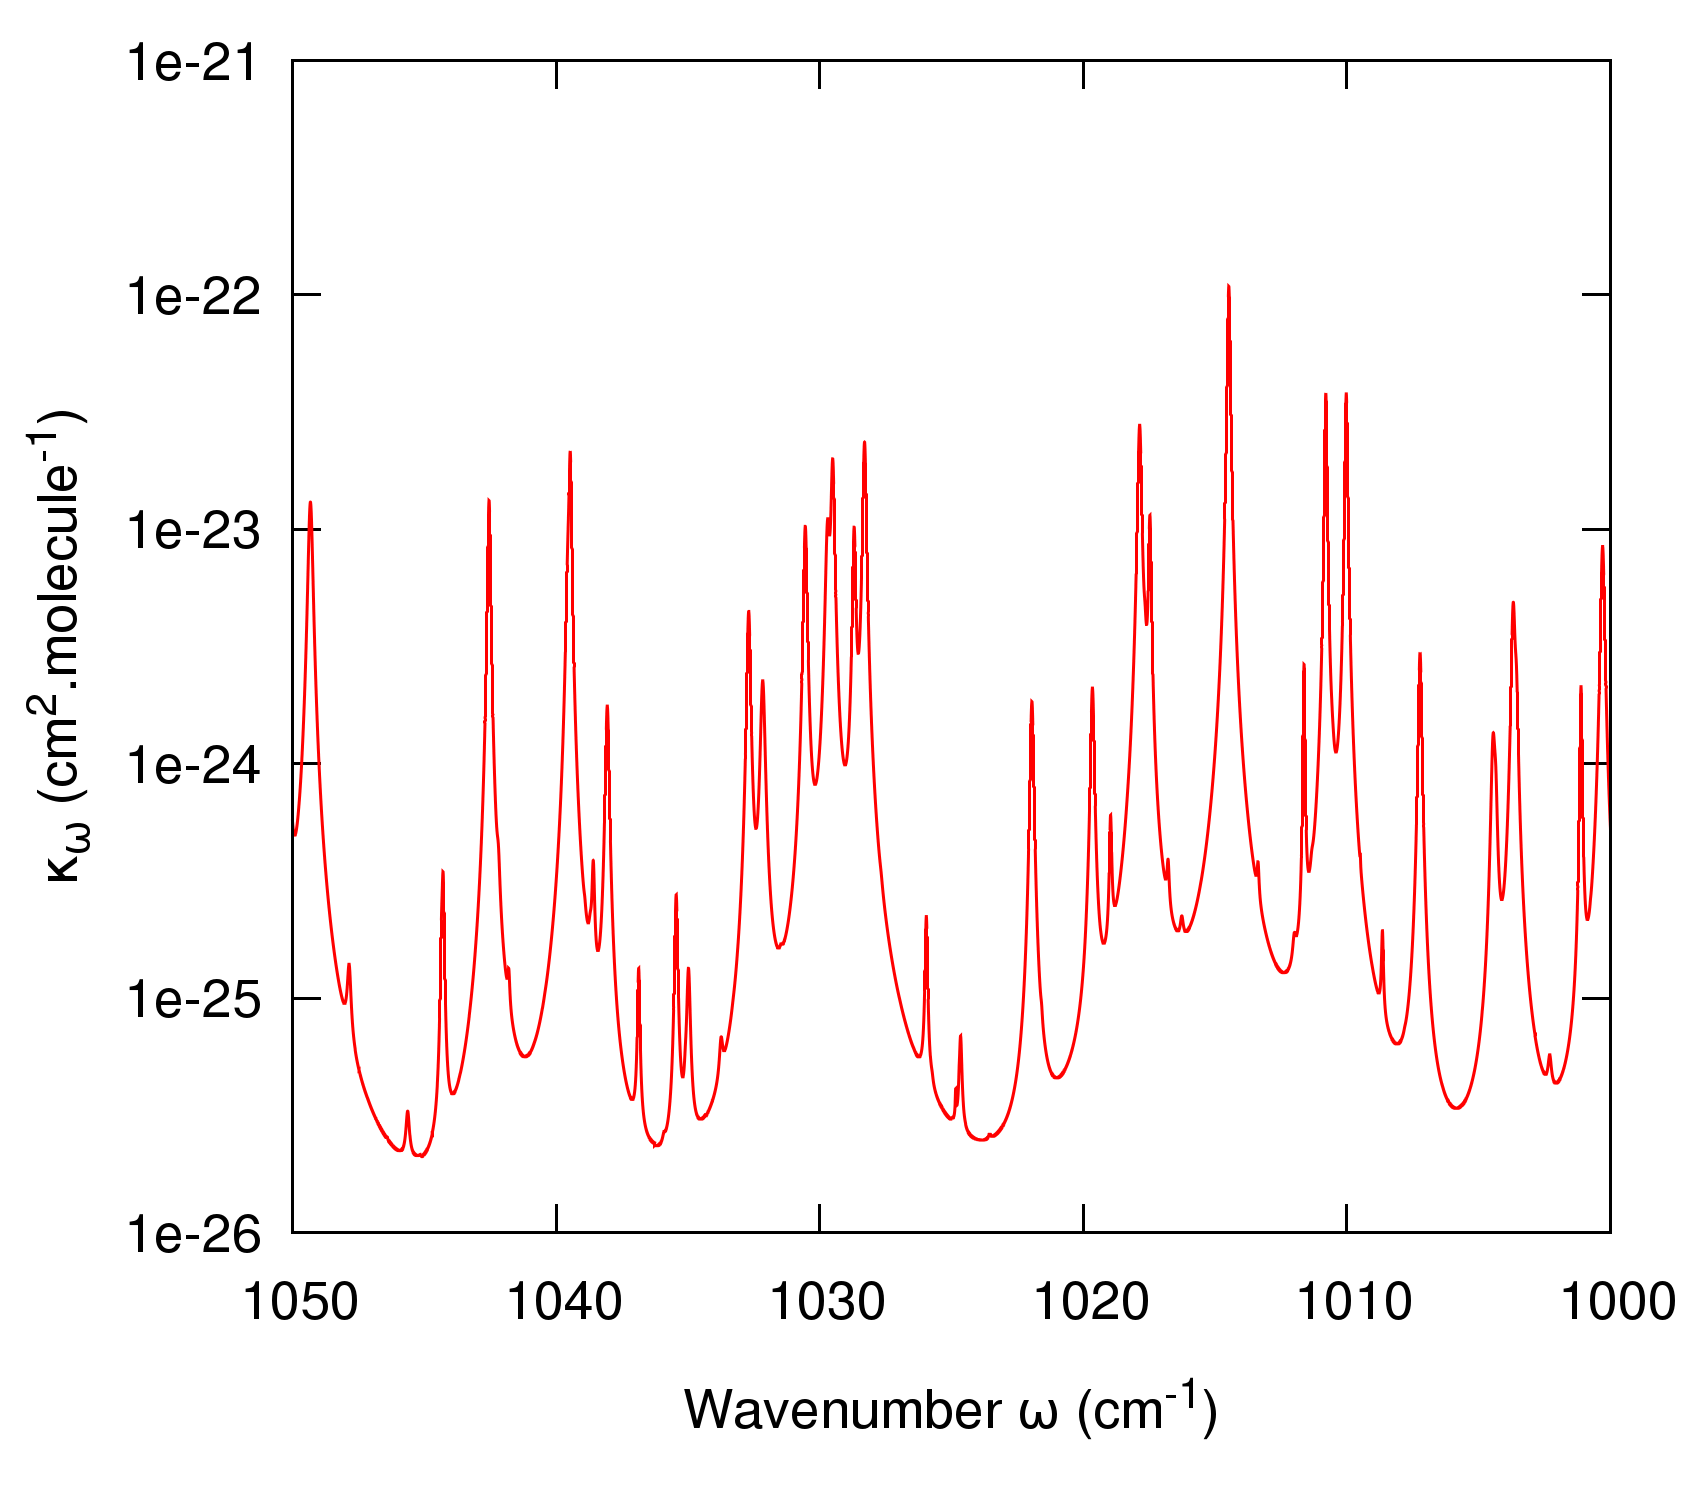
\includegraphics[width=4.0in]{Figures/H20_Line_Strength.png}
\end{center}
 \caption{Spectral $\rm H_2O$ absorption coefficient $\kappa_{\om}$ for the spectral range 1000 -- 1050~cm$^{\rm -1}$. This synthetic spectrum calculated using HITRAN 2012 line specifications assumes a temperature of 296~K and 10\% of water in a total pressure of 1~atm.\label{fig:H2O_Detailed_spectrum}}
\end{figure}

\subsection{Planck blackbody distribution law}

The Planck blackbody distribution law, sometime called the Planck function, but the term is misleading as it is a distribution, describes the spectral distribution of the equilibrium rate of radiant energy emitted from a blackbody at temperature $T$. Its expression is given, as a function of frequency $\nu$ and for an unit of solid angle, by:
\begin{equation}\label{eq:Plank_freqency}
I_{\rm b,\nu}(T) = \displaystyle\frac{2 h\nu^3}{c^2}\displaystyle\frac{1}{\exp\left(\displaystyle\frac{h\nu}{k_{\rm B}T}\right)-1}.
\end{equation}
Here, $h$ is the Planck constant ($6.626 \times 10^{-34}$~J$\cdot$s), and $k_{\rm B}$ is the Boltzmann constant ($1.381 \times 10^{-23}$~J/K). $I_{\rm b,\nu}(T)$ is in units of $\rm{W/m^{2}/str/s^{-1}}$.

In terms of wavenumber, the Planck blackbody distribution law, $I_{\rm b,\om}$, is written:
\be\label{eq:Planck_WN}
I_{\rm b,\om}(T) = \dfrac{2 \, h \, c^2 \, \om^{3}}{\exp\left(\dfrac{h \, c\, \om}{k_{\rm B} \, T }\right)-1} .
\ee
$I_{\rm b,\om}(T)$ is in units of $\rm{W/m^2/str/m^{-1}}$; the wavenumber $\om$ in Eq.~\ref{eq:Planck_WN} is in units of $\rm{m^{-1}}$.

The user who wishes to express the Planck blackbody distribution law as a function of wavelength should take caution when performing the change of variables. One should start by expressing that the radiant energy emitted at a wavelength $\la$ over an infinitesimal spectral range $\d\la$ is the same as the radiant energy emitted at the corresponding wavenumber $\om$ over an infinitesimal spectral range $\d\om$:
\be \label{eq:Planck_WN_WL}
I_{\rm b,\la}(T) \d \la = -I_{\rm b,\om}(T)\d \om,
\ee
the negative sign is introduced because $\om$ is the reciprocal of $\la$. Since $\la$ = 1/$\om$, it comes:
\be
\dfrac{\d \la}{\d \om} = -\dfrac{1}{\om^2}.
\ee
Equation \ref{eq:Planck_WN_WL} can be rewritten, after the appropriate change of variables:
\be \label{eq:Planck_WL}
I_{\rm b,\la}(T) = \dfrac{2 \, h \, c^2}{\la^5}\dfrac{1}{\exp\left(\dfrac{h \, c}{\la \, k_{\rm B} \, T }\right)-1},
\ee
where $I_{\rm b,\la}$ is in units of $\rm{W/m^2/str/m}$; the wavelength $\la$ in Eq.~\ref{eq:Planck_WL} is in unit of $\rm m$.

\begin{figure}
\begin{center}
 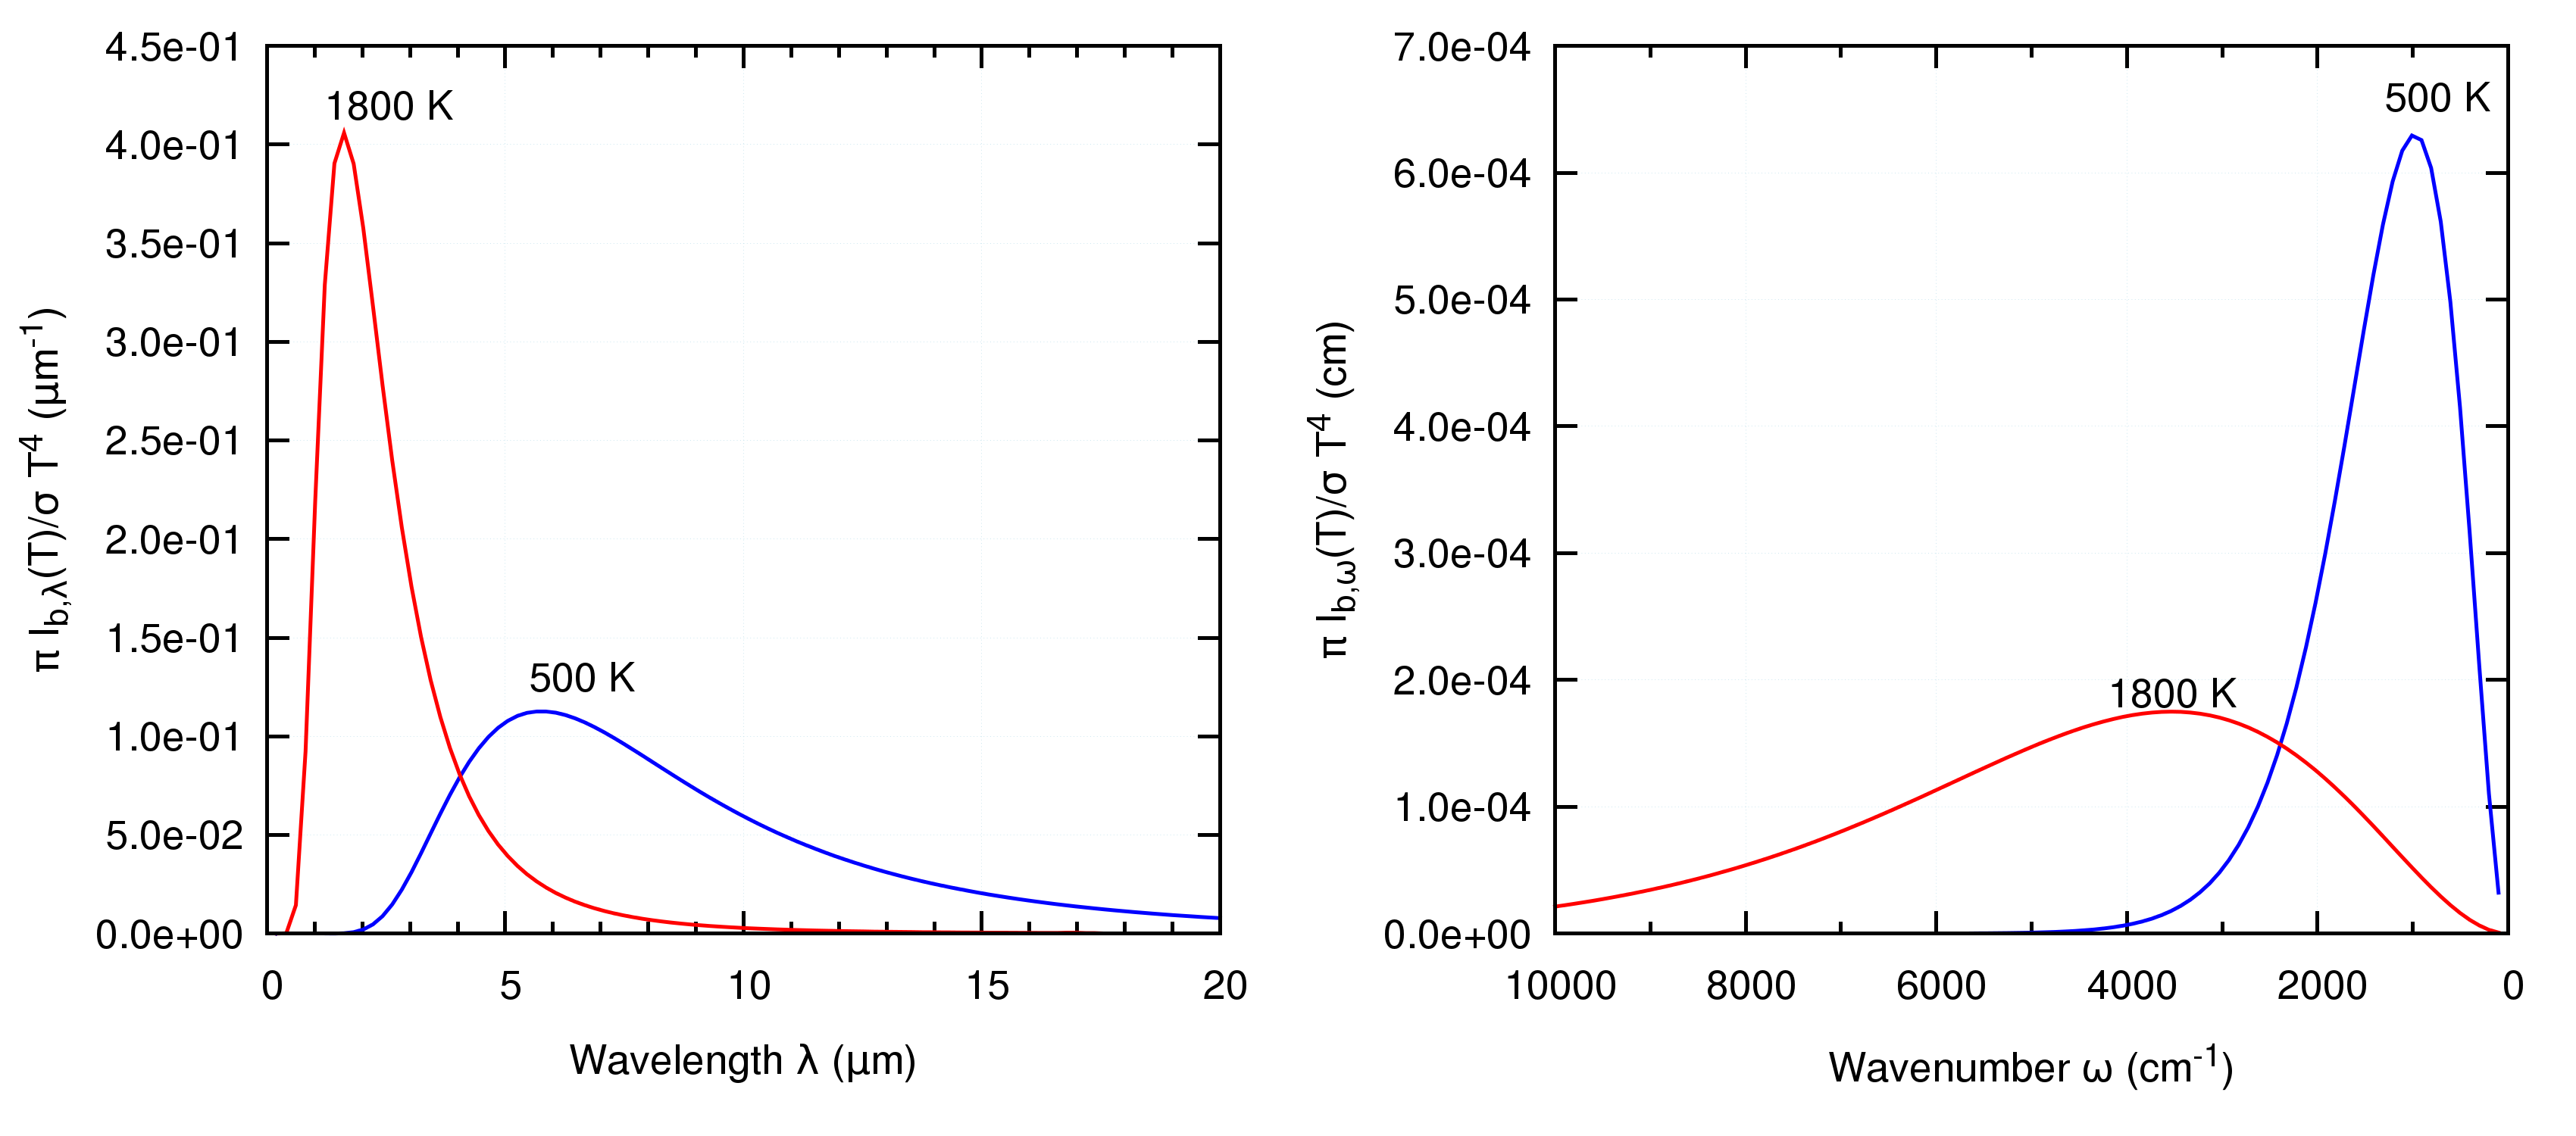
\includegraphics[width=6.5in]{Figures/Black_body.png}
\end{center}
 \caption{Normalized spectral Blackbody distributions at T = 500~K (blue line) and T = 1800~K (red line) with the wavelength in units of $\mu m$ (left) and with the wavenumber in units of $\rm cm^{-1}$ (right). \label{fig:bb_spectrum}}
\end{figure}

Figure~\ref{fig:bb_spectrum} plots profiles of normalized spectral Blackbody distribution for temperatures of 500~K and 1800~K using wavelength and wavenumber. It can be seen that an increase of temperature will shift the mode of the distribution toward lower wavelength and higher wavenumber. Figure~\ref{fig:bb_spectrum} indicates that the shape of the distribution is not invariant with the units chosen to characterize the spectrum. Indeed, while an elevation of blackbody temperature corresponds to a narrowing of the normalized distribution when using wavelength, the same elevation of blackbody temperature leads to a spreading of the profile when using wavelength. Finally, an important remark is that the location of the distribution mode (corresponding to the location of maximum emission) does not relate between wavelength and wavenumber. This location can be calculated using the Wien's displacement law. Using wavelength, the Wien's displacement law is expressed by:
\begin{equation}\label{eq:Wien_WL}
\la_{\rm max} T = 2898 \; \mu \rm m . \rm K,
\end{equation}
while using wavenumber, the Wien's displacement law is expressed by:
\begin{equation}\label{eq:Wien_WN}
 \dfrac{\om_{\rm max}}{T} = 1.961 \; \rm cm^{-1}.K^{-1}.
\end{equation}
Using Eq.~\ref{eq:Wien_WL}, the maximum of emission at 500~K is located at $\la_{\rm max} = \rm 5.8 \; \mu m$. The same calculation using Eq.~\ref{eq:Wien_WN} gives $\om_{\rm max} =  980 \; \rm cm^{-1}$. It is crucial to note that $10000/\la_{\rm max} = 1725 \; \rm cm^{-1} \; \neq \om_{\rm max}$. Hence caution must me taken when converting spectral variable from wavenumber to wavelength and vice versa. In RadCal, the wavenumber is the variable of choice for spectral quantities.

\section{Single line emission}
This section briefly recalls the characteristics of a single line emission. The expression for an isolated line with pressure broadening mechanism (also called Lorentz lines) is recalled along with the expression of lines broadened by Doppler effects. Note that RadCal mixes both lines expression in the calculation of the RTE. Hence, it is important to recall some of their properties. The underlying mechanisms responsible for the emission and/or absorption of electromagnetic radiation by a molecule or atom are not recalled here as they are out of the scope of this work. It is just recalled here that the discrete nature of a species spectrum in the infrared region is a direct consequence of the discretization of the vibrational and rotational energy level admissible for a given species. The location and intensity of these lines can be obtained from the solution of the time-dependent Schr\"{o}dinger wave equation of a molecule with an incident radiation field. The lines location and intensity depend on the molecule geometry, mass, and its electric dipole moments. For further details, see Chapter 7 of Penner, Ref.~\cite{Penner1959}; Herzberg Ref.~\cite{Herzberg1949}; Chapter 11 of Modest, Ref.~\cite{Modest2013}; and Tien monograph Ref.~\cite{Tien1968}.

\subsection{Lorentz lines}
A spectral line is never truly monochromatic as different line broadening mechanisms are present. The most fundamental one is the natural line broadening which is a consequence of the Heisenberg's uncertainty principle. While this effects is always present, it is usually omitted in engineering applications as the collision broadening and the Doppler broadening mechanisms are much more important.

The collision broadening mechanism originates from disruptions during the emission or absorption of energy due to the collision between molecules. The broadening of the line increases as the collision frequency increases, hence as the local pressure is increased. The shape of such broadened lines can be calculated using the electron theory of Lorentz or from quantum mechanism. The shape of the line is given by:
\begin{equation}\label{eq:lorentz_line}
 \kappa_{\om} = \dfrac{S}{\pi}\dfrac{\gamma_c}{\left( \om - \om_o\right)^2 + \gamma_c^2},
\end{equation}
where $\gamma_c$ is the collision broadening half-width at half the maximum (HWHM), $\omega_0$ is the wavenumber at the line center, and $S$ is called the line intensity or line strength and is defined as:
\begin{equation}
 S = \displaystyle\int{\kappa_{\om} \d \om}.
\end{equation}
Note that $S$ is a function of the temperature alone while $\gamma_c$ is a function of the temperature, pressure, and mixture composition. Because the effects of collision depend on the molecular diameters of the colliding species, the quantity $\gamma_c$ varies with the collisional partner. Among the collision broadening, distinction is made between the foreign gas broadening, \textit{i.e.} due to collisions among dissimilar species, and self-broadening, \textit{i.e} due to collisions among like species. The self-broadening collisions can be further differentiated between resonant and non-resonant collisions. Resonant collisions are more effective than non-resonant collisions but they have a different temperature dependence than non-resonant collisions. Non-resonant collisions are similar to collisions with a foreign gas. In RadCal, when not tabulated, the Lorentz HWHM $\gamma_{c,i}$ of a given species $i$ belonging to a mixture, is calculated according to:
\begin{equation}\label{eq:gamma_L}
 \gamma_{c,i} = \displaystyle\sum_{j} \gamma_{c0,(i,j)} \left(\dfrac{P_j}{P_0}\right)\displaystyle\sqrt{\dfrac{T_0}{T}} + \gamma^*_{c0,i}\dfrac{P_i}{P_0}\left(\dfrac{T_0}{T}\right),
\end{equation}
where $\gamma_{c0,(i,j)}$ denotes the value of non-resonant collision broadening HWHM with species $j$ at conditions of standard pressure (denoted $P_0$) and temperature (denoted $T_0$), and $\gamma^*_{c0,i}$ demotes the value of resonant self-collision broadening HWHM at conditions of standard pressure and temperature. Note that Eq.~\ref{eq:gamma_L} first right-hand side term includes the effects of foreign gas collision and non-resonant self-collision.

Profile of a normalized Lorentz line ($\kappa_{\omega} (\pi \gamma_c)/S$ as a function of $(\omega-\omega_0)/\gamma_c $) is plotted in Fig.~\ref{fig:Lorentz_line} together with the profile of a normalized Doppler line.

\begin{figure}
\begin{center}
 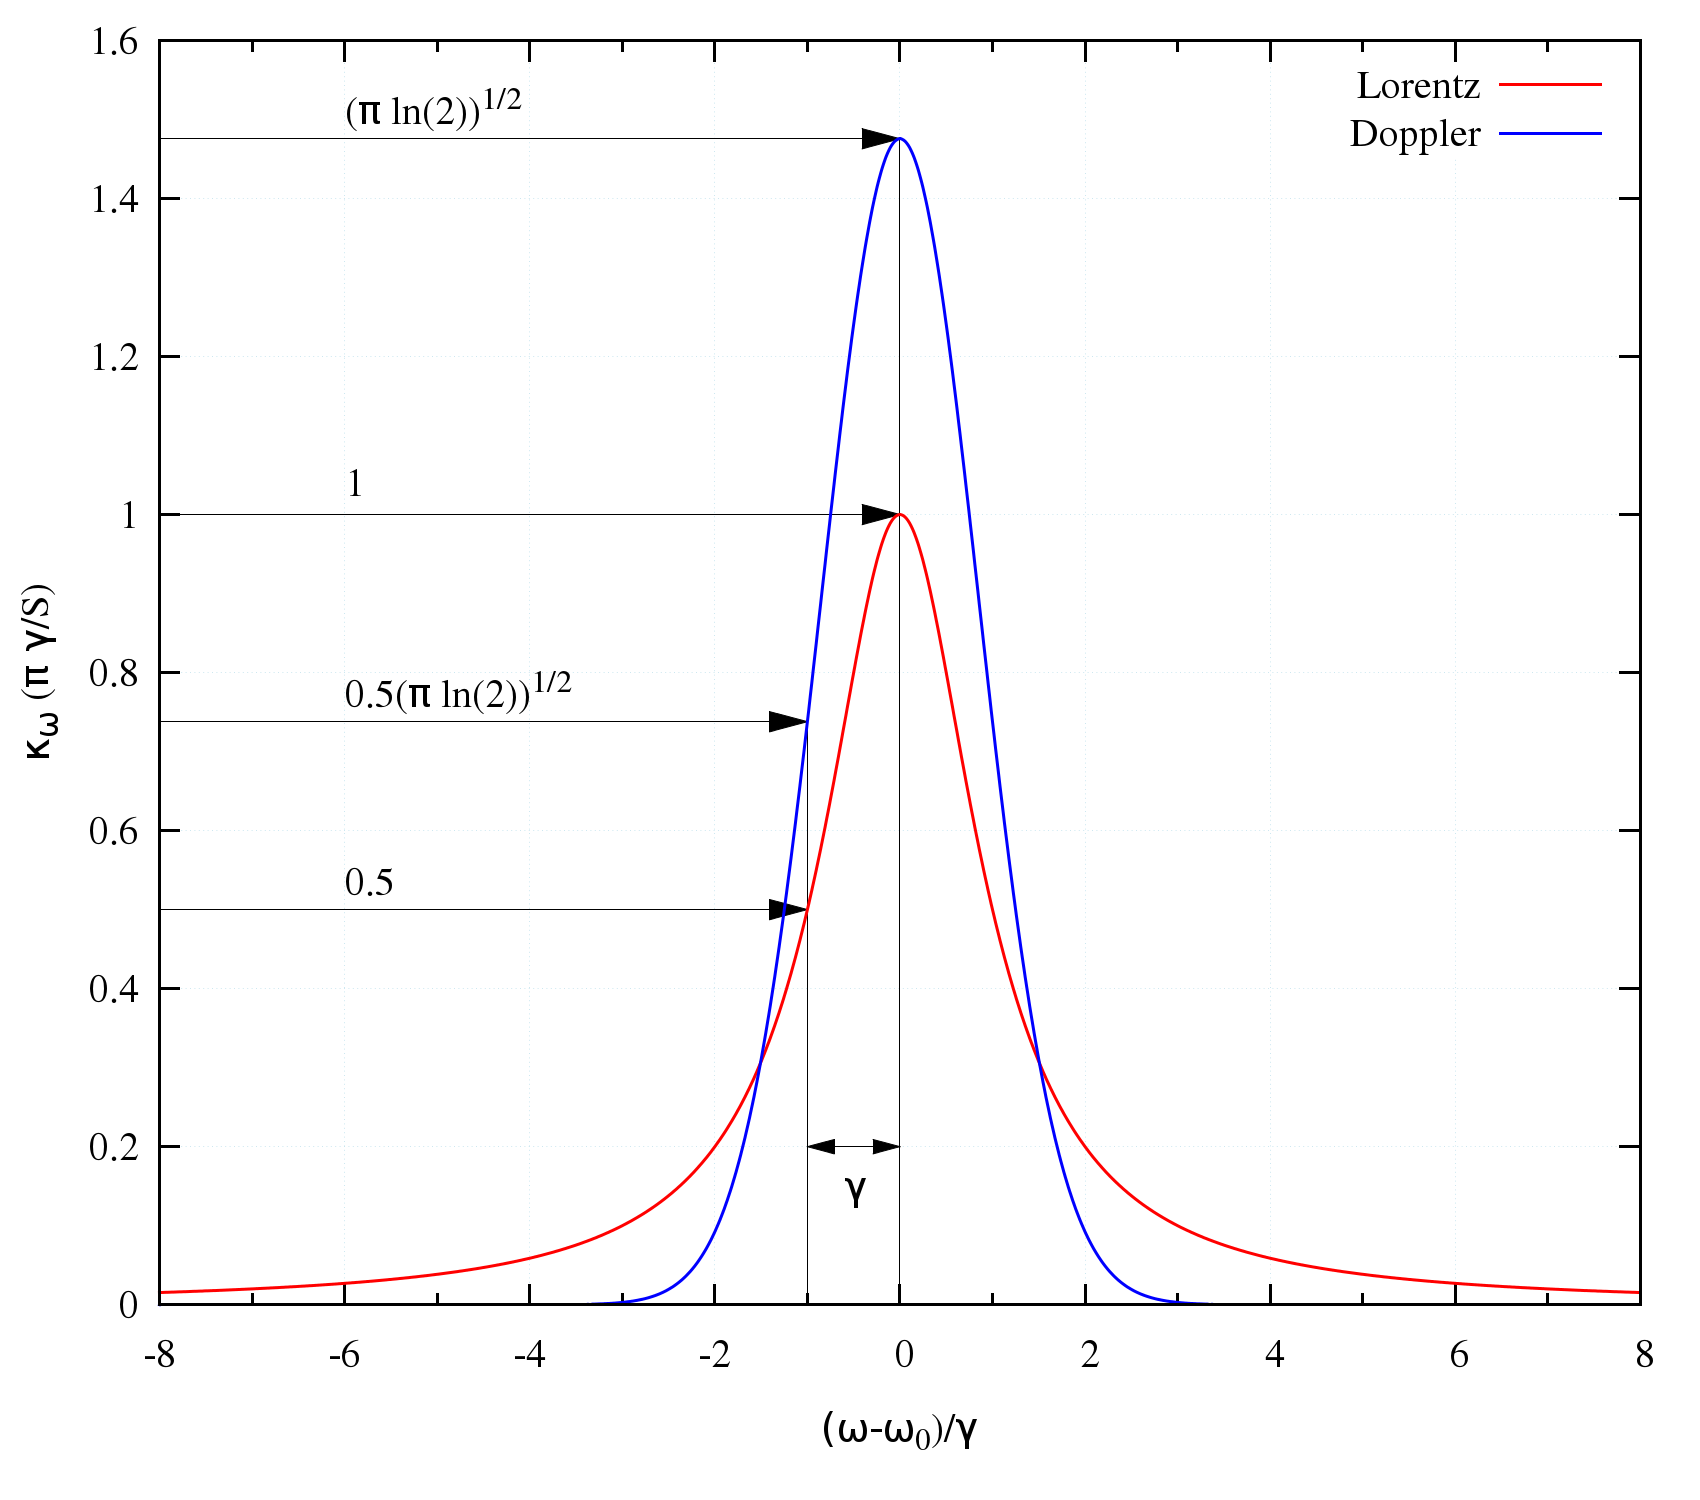
\includegraphics[width=4.0in]{Figures/Lorentz_Doppler.png}
\end{center}
 \caption{Profiles of a normalized Lorentz line (in red) and a normalized Doppler line (in blue). \label{fig:Lorentz_line}}
\end{figure}

\subsection{Doppler lines}
The motion of radiating particles in the line of sight may change the apparent frequency due to the Doppler effect. The apparent frequency increases when the particle moves toward the observer and decreases when it moves away. The Doppler line profile is calculated considering the Maxwell velocity distribution (which is a consequence of the local thermodynamic equilibrium assumption). The absorption coefficient is then expressed as:
\begin{equation}
\kappa_{\omega} = S \dfrac{\displaystyle\sqrt{\rm ln(2) }}{ \gamma_D \displaystyle\sqrt{\pi} } \exp{\left[- \rm ln(2) \left( \dfrac{\omega-\omega_0}{\gamma_D} \right)^2 \right]},
\end{equation}
where $S$ and $\omega_0$ are the line strength and the wavenumber at the line center, respectively. The quantity $\gamma_D$ is the Doppler HWHM. It is calculated from:
\begin{equation}\label{eq::DopplerHWHM}
  \gamma_D = \displaystyle\frac{\omega_0}{c} \displaystyle\sqrt{\rm{ ln(2)} \displaystyle\frac{2 k_B T}{m} },
\end{equation}
where $m$ is the mass of the radiating species. Note that the Doppler HWHM depends linearly on the wavenumber; it increases with elevated wavenumber.
The Doppler broadening mechanism is important at high temperature ($T > 2000\;K$) \cite{Modest2013} and/or low pressure, typically lower than 0.01 atm.
In RadCal both broadening mechanisms are included in the calculation of the RTE; see Section~\ref{sec:RTE_NB}.

\subsection{Emission from an isolated line}
This subsection recalls the results of the emission and absorption of radiation for an isolated Lorentz line. This ideal case helps to bring an understanding of a single line absorption variation with the pressure path length as it is a very fundamental concept.

The spectral variation of the absorption coefficient $\kappa_{\om}$ of a single line centered in $\om_0$, of line strength $S$, and of HWHM $\gamma_c$ with the wavenumber $\om$ is recalled:
\begin{equation}
 \kappa_{\om} = \dfrac{S}{\pi}\dfrac{\gamma_c}{\left( \om - \om_o\right)^2 + \gamma_c^2}. \tag{\ref{eq:lorentz_line}}
\end{equation}
The shape of the line is plotted in Fig.~\ref{fig:Lorentz_line}.

Assuming a path going through an isothermal gas, of temperature $T_g$, and homogeneous layer of participating species of partial pressure $P_i$, and of physical thickness $L$, the RTE, Eq.~\ref{eq:RTE_Final}, can be simplified as:
\begin{equation}
 I_{\om}(L) =  I_{\om}(0) \exp\left( -\kappa_{\om} P_i L\right) + I_{\rm b,\om}\left(T_g\right) \left(1-\exp\left(-\kappa_{\om} P_i L\right)\right).
\end{equation}
Note that in this equation, the local amount of participating species is expressed by the partial pressure $P_i$; hence in the equation above, $\kappa_{\om}$ has the dimension of an inverse pressure times an inverse length. In RadCal, $\kappa_{\om}$ is expressed in $\rm (cm^{-1} \cdot atm^{-1})$, while $P_i$ is in $\rm atm$ and the path physical length $L$ is in $\rm cm$. The product $P_i\;L$, the pressure path length, is referred to in RadCal as a species optical thickness and is also denoted $U$, and the product $\kappa_{\om}\;P_i\;L$ is referred to as the optical depth.

Considering only the emission term (\textit{i.e.} $I_{\om}(0)$ = 0), the exiting intensity integrated over the whole spectrum, emitted by a single line, denoted $I(L)$, is expressed as:
\begin{equation}
I(L) =  I_{\rm b,\om}\left(T_g\right) \displaystyle\int_{\Delta \om}\left( 1-\exp\left(-\kappa_{\om'} P_i L\right)\d \om'\right),
\end{equation}
this assumes that $I_{\rm b,\om}$ does not vary much over the $\Delta \om$ range. The integrand is often called the equivalent line width \cite{Modest2013} and is usually denoted $W$,
\be
W = \displaystyle\int_{\Delta \om}\left( 1-\exp\left(-\kappa_{\om'} P_i L\right)\d \om'\right).
\ee

The analytical expression of $W$ for a Lorentz line can be derived, see for example Penner, \cite{Penner1959}:
\be
W(P_i L) = 2 \pi \gamma_c L(x) = 2  \pi \gamma_c x \;\exp\left( -x\right) \left(I_0(x) + I_1(x)\right), \; x = \dfrac{SP_iL}{2 \pi \;\gamma_c}.
\ee
The function $L(x)$ is named the Ladenburg-Reiche function, and $I_0$ and $I_1$ are the modified Bessel functions of the first kind. The graph of the Ladenburg-Reiche function is
given in Fig.~\ref{fig:Ladenburg}. Note that for small and large values of $x$, the equivalent line has the following asymptotic forms:
\begin{align}
W(x) \sim SP_iL ,\: {\rm for}\: x \ll 1 \\
W(x) \sim 2\sqrt{S\gamma_c P_iL} ,\: {\rm for}\: x \gg 1.
\end{align}

\begin{figure}
\begin{center}
 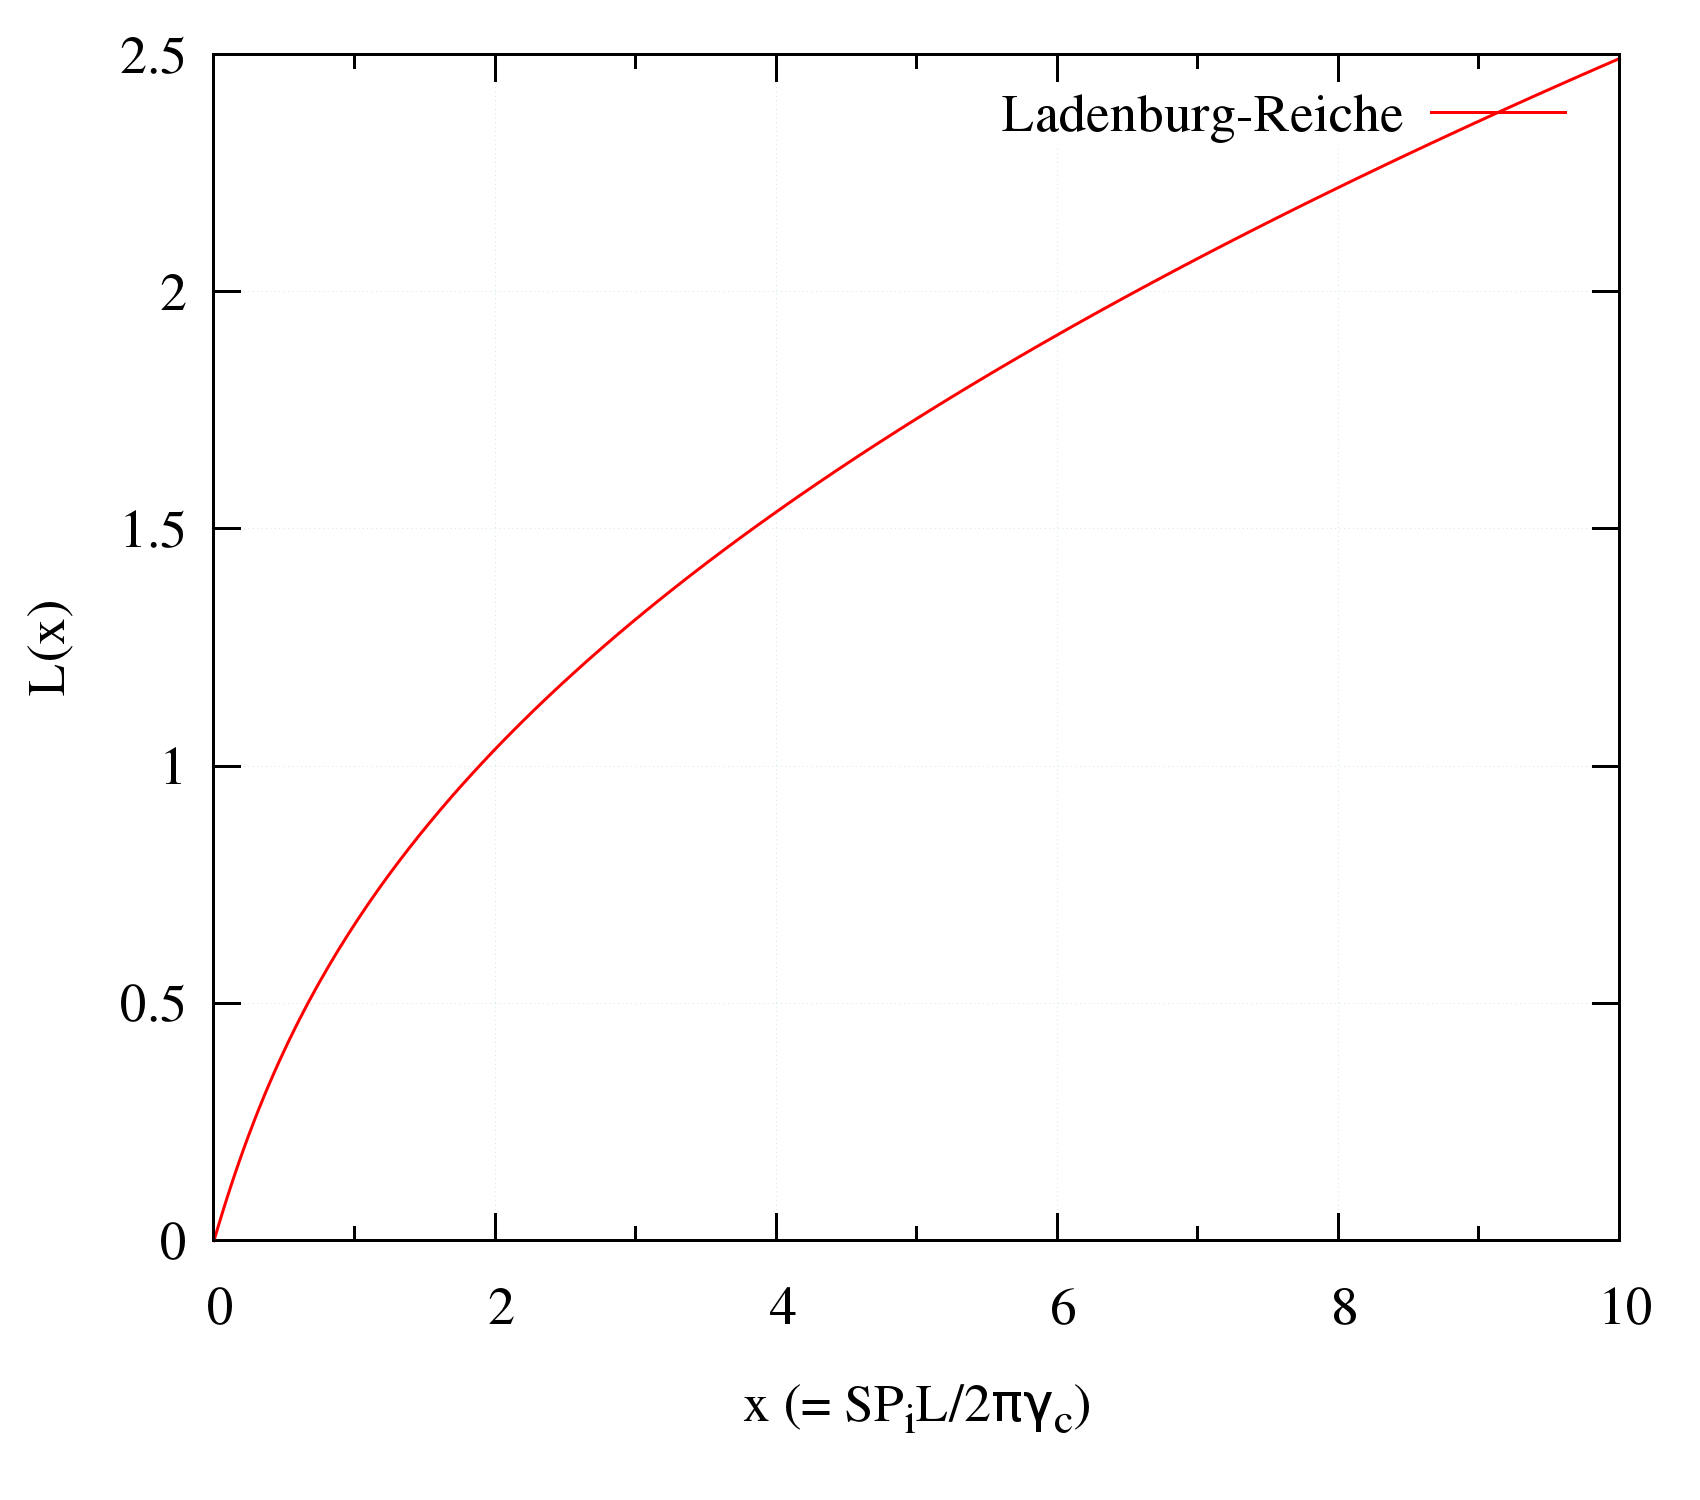
\includegraphics[width=4.0in]{Figures/Ladenburg.png}
\end{center}
 \caption{Profile the Ladenburg-Reiche function. \label{fig:Ladenburg}}
\end{figure}

It is worth noting that the parameter $x$ gives an indication of the optical thickness of the gas layer for a single line. When $x$ is small, this indicates that the medium is weakly participating (either $S$ or the product $P_iL$ is small) and the absorption and emission of a single line is linear with the product $P_iL$. On the contrary, when $x$ is much greater than unity, the absorption or emission of a single line is not linear anymore but has a square-root dependency.

\section{Narrow band models}\label{Sec::SNBM}
This section briefly describes the different models used to obtain most of the tabulated species IR spectral mean absorption coefficients at different temperatures, $\bar{\kappa}_i(\om,T)$. Narrow band models are used in lieu of line-by-line models to represent the IR spectra of radiating species in engineering applications. In the narrow-band approach, the whole spectrum is divided into small spectral bands (typically several $\rm cm^{-1}$), and different statistical approaches are used to compute the average radiative properties over these narrow-bands. What is of interest is to give functional expression of the integrand:
\be
\bar{\tau}_{\om} = \displaystyle\int_{\Delta \om}\left( \exp\left(-\kappa_{\om'} P_i L\right)\d \om'\right),
\ee
when $\Delta \om$ is large enough so it includes hundreds, even thousands, of single lines, but small enough to assume $I_{\rm b,\om}\left(T_g\right)$ and the incident spectral intensity $I_{\om}(0)$ constant over it. It is important to state that generally:
\be
\bar{\tau}_{\om} \neq \displaystyle\int_{\Delta \om}\left( \exp\left(-\bar{\kappa}_{\om'} P_i L\right)\d \om'\right).
\ee
Equality is verified only is some specific situations (\textit{e.g.} $P_iL \ll 1$). An important assumption to recall is that it is assumed that the Kirchoff law, \textit{i.e.} $\bar{\alpha} = \bar{\epsilon}$, holds over a narrow-band.

Three main narrow-band models are presented below: the Elsasser model, the Goody model, and the Malkmus model. All assume Lorentz lines.

\subsection{Elsasser model}

The Elsasser model assumes all the lines to have the same HWHM $\gamma_c$, the same line strength $S$, and to be equally spaced every $d$ wavenumber from each other.
As a consequence, the absorption coefficient can be expressed by the infinite sequence:
\be\label{eq:kappa_El}
\kappa_{\om} = \displaystyle\sum_{n = -\infty}^{\infty}{\dfrac{S}{\pi}\dfrac{\gamma_c}{\left(\om - \left(\om_0+n\,d\right)\right)^2 + \gamma_c^2}}.
\ee
This function is periodic, with a period $d$. Following Elsasser derivation (see Ref.~\cite{Penner1959}), Eq.~\ref{eq:kappa_El} can be expressed as:
\be\label{eq:Elsasser_periodic}
\kappa_{\om}  = \dfrac{S}{d} \dfrac{\rm sinh (8\beta)}{{\rm cosh (8\beta)} - \cos(\frac{2\pi}{d}(\om-\om_0))},
\ee
where the overlap parameter $\beta$, which is also called the (Lorentz) fine structure parameter and denoted $a_c$ in Ref.~\cite{Ludwig1973} and in the code, is defined here as:
\be\label{eq::beta}
\beta = \dfrac{\pi}{4}\dfrac{\gamma_c}{d}.
\ee
The mean absorption coefficient $\bar{\kappa}$ over the narrow-band centered in $\om$ is:
\be\label{eq:kappa_def}
\bar{\kappa}_{\om} = \dfrac{S}{d}.
\ee
Figure~\ref{fig:Elsasser_profile} plots the variations of the Elsasser absorption coefficient $\kappa_{\om}$ normalized by $\bar{\kappa}$ as a function of the ratio $\om/d$ for two different values of the overlap parameter $\beta$. Strong overlap effects are seen for the largest value of $\beta$.

\begin{figure}
\begin{center}
 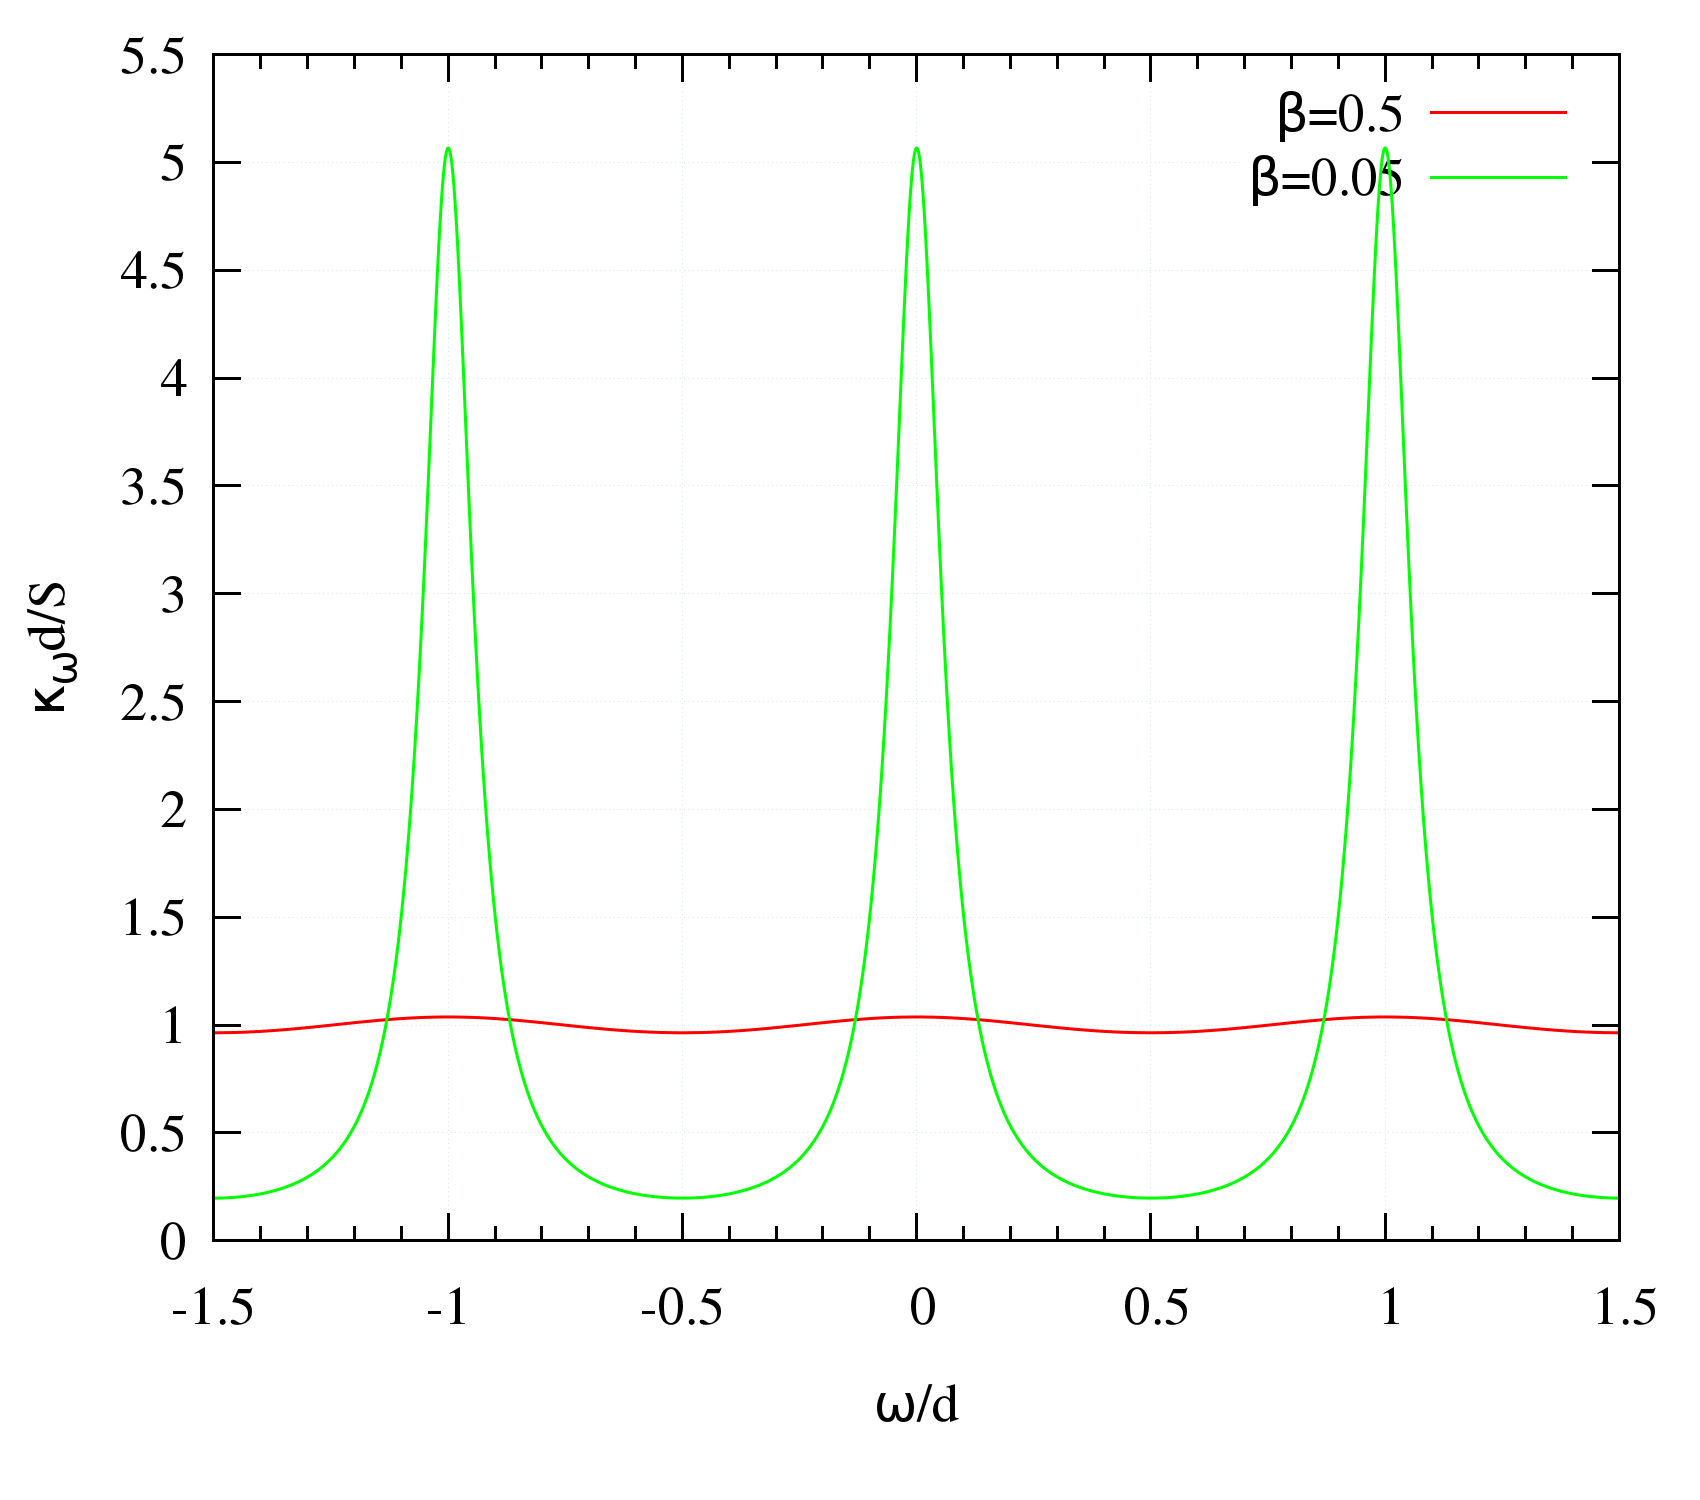
\includegraphics[width=4.0in]{Figures/Elsasser_profile.png}
\end{center}
 \caption{Variations of the Elsasser absorption coefficient normalized by $\bar{\kappa}$ plotted as a function of the ratio $\om/d$ for two different values of the overlap parameter $\beta = 0.05$ (in green) and $\beta = 0.5$ (in red). \label{fig:Elsasser_profile}}
\end{figure}
The mean transmissivity $\bar{\tau}_{\om}$ of the narrow-band centered in $\om$ can be calculated using Eq.~\ref{eq:Elsasser_periodic}, averaging over one period $d$:
\be
\bar{\tau}_{\om} = \frac{1}{d}\displaystyle\int_{-\frac{d}{2}}^{\frac{d}{2}}{\exp\left(-\bar{\kappa}_{\om} P_i L\dfrac{\rm sinh (8\beta)}{{\rm cosh (8\beta)} - \cos\left(\frac{2\pi}{d}(\om'-\om)\right)} \right)\d\om'}.
\ee
This expression can be assessed using the Godson and Tien approximations \cite{Brosmer1985b,Kunitomo1975}:
\be\label{eq::Elsasser}
    \bar{\tau}_{\om} = 1- \erf \left( \dfrac{\sqrt{\pi}}{2} \, \frac{\bar{\kappa}_{\om} \, U }{\displaystyle \sqrt{1 + \frac{\pi \, \bar{\kappa}_{\om} \, U}{16 \, \beta}}}  \right),
\ee
where $U = P_iL$ is the optical thickness. Equation~\ref{eq::Elsasser} is used in RadCal to compute $\bar{\tau}_{\om}$ when using the Elsasser narrow-band model, which is only used for Methane. Note that the Godson and Tien approximation is reasonably accurate for values of the overlap parameter lower or of the order of unity, \textit{i.e.} $\beta < 1$.
Figure~\ref{fig::Elsasser_curve_growth} plots the quantity $-\ln(\bar{\tau}_{\om})$ (this quantity is also referred to as the curved of growth) versus the product $\bar{\kappa}_{\om} U$ for two different values of the overlap parameter: $\beta = 0.05$ (in green) and $\beta = 0.5$ (in red). The back dashed curve corresponds to the ``linear'' behavior, \textit{i.e.} $\bar{\tau}_{\om} = \exp\left(\bar{\kappa} U\right)$. It is noteworthy that this linear behavior corresponds to either ``weak lines regimes'' (situations with small product $\bar{\kappa} U$) or to situations with a strong overlap, $\beta > 1$). Outside of these regimes, assuming linear behavior might lead to overestimation of the curve of growth. Figure~\ref{fig::Elsasser_curve_growth} also illustrates a case where the Godson and Tien approximation looses its accuracy and leads to unphysical results, as seen for the case $\beta=0.5$, which overestimates the absorption.

It can be seen from Eq.~\ref{eq::Elsasser} that $\bar{\tau}_{\om}$ is fully characterized once the narrow-band parameters $\bar{\kappa}_{\om}$ and $\beta$ are known. Note that these two parameters are by construction independent of the physical length of radiation propagation but depend on the local temperature, pressure, and local mixture composition.

\begin{figure}
\begin{center}
 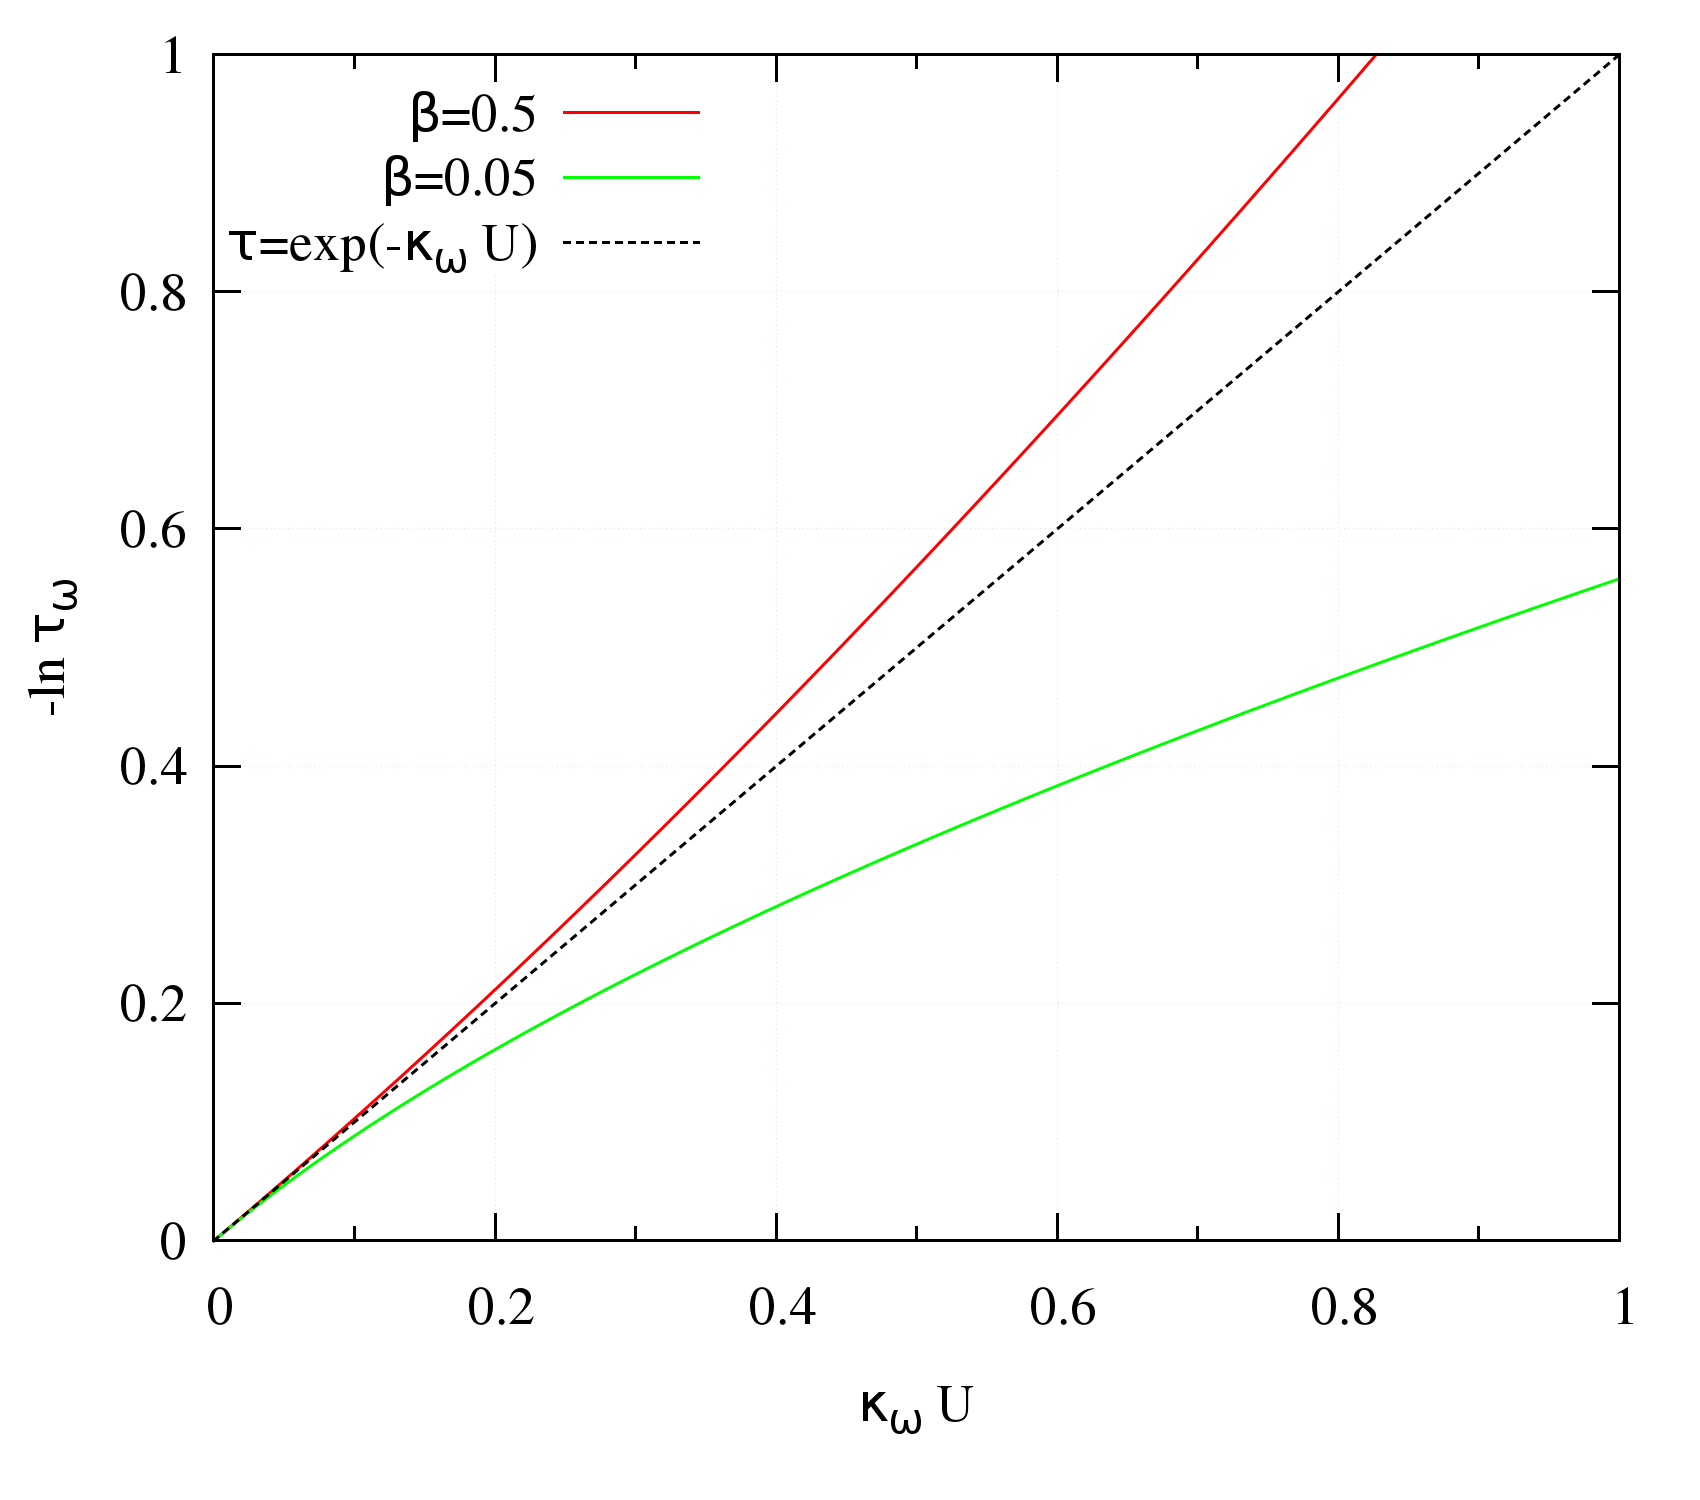
\includegraphics[width=4.0in]{Figures/Elsasser_curve_of_growth.png}
\end{center}
 \caption{Elsasser model curve of growth ($\ln \bar{\tau}$) as a function of the product $\bar{\kappa}_{\om} U$. Two different values of the overlap parameter are plotted: $\beta = 0.05$ (in green) and $\beta = 0.5$ (in red). The curve of growth for the ``weak line regime'' is plotted in the bash dashed curve.\label{fig::Elsasser_curve_growth}}
\end{figure}

\subsection{Generalities on statistical narrow-band models}
The Goody and Malkmus models have been developed to provide a better modeling of the narrow-band spectral properties than that predicted by the Elsasser model, which is based on strong assumptions: uniformity of the line strength and of line spacing. While the Elsasser model works fine for some light, diatomic  species (\textit{i.e} HCl), most of the more complex polyatomic species cannot be modeled appropriately with the Elsasser model, since the very detailed experimental characterization of their spectral lines does not exhibit regularity \cite{Modest2013}.

The Goody and Malkmus models are statistical narrow-band models, the former preceding the latter by a couple of decades and was first developed by Mayer and Goody \cite{Penner1959}. Statistical narrow-band models are based on two main assumptions: first, there is no correlation between lines position and line intensities, and the location of the line can be modeled by any random arrangement~\cite{Penner1959,Young1977d}; second, while all the lines have the same shape, their line strength within the narrow-band of spectral range $\Delta \nu$ is a random variable assigned to a continuous probability density function $P(\bar{S},S)$, with $\bar{S}$ the mean value of the line strength, \textit{i.e.} $\bar{S} = \displaystyle\int_{0}^{+\infty}{S P(\bar{S},S)\d S}$.

A consequence of these assumptions for a very large number of lines contained within the narrow-band is that the transmissivity of a narrow-band $\bar{\tau}_{\om}$, and of optical thickness $U$, is expressed by:
\be\label{eq:SNB_tau_equiline}
\bar{\tau}_{\om}(U) = \exp\left(-\displaystyle\frac{\bar{W}(U)}{d}\right),
\ee
where $d$ is the average line spacing and $\bar{W}(U)$ is the average equivalent line width of the narrow-band considered and is calculated as:
\begin{align}\label{eq::SNB_Equiline}
\bar{W}(U) &= \displaystyle\int_{0}^{+\infty}{P(\bar{S},S)W(S,U) \d S} \nonumber \\
           &= \displaystyle\int_{0}^{+\infty}{P(\bar{S},S)\displaystyle\int_{-\infty}^{+\infty}{1 - \exp\left(-\kappa_{\om} P_i L\right) \d\om} \d S}
\end{align}
where $\kappa_{\om}$ is the absorption coefficient of a Lorentz line, given by Eq.~\ref{eq:lorentz_line}. An example of the derivation of Eq.~\ref{eq::SNB_Equiline} is presented in Penner's book~\cite{Penner1959}. By their different choice of the probability density function $P(\bar{S},S)$, the Goody and Malkmus models provide an explicit and simple evaluation of the average equivalent line width of a narrow-band, $\dfrac{\bar{W}}{d}$.

\subsection{Goody model}\label{sec:goody_model}

The Goody model assumes an exponential distribution of the line strength:
\begin{align}
 P(\bar{S},S) &= \dfrac{1}{\bar{S}}\exp\left(-\dfrac{S}{\bar{S}} \right) \\
              &= \dfrac{4}{\pi S_E}\exp\left(-\dfrac{4S}{\pi S_E} \right),
\end{align}
where $S_E$ is an effective equivalent line strength which relates to the average line strength $\bar{S}$ with \cite{Malkmus1967,Ludwig1973}:
\be\label{eq::S_E_barS}
\bar{S} = \dfrac{\pi}{4} S_E.
\ee
Solving Eq.~\ref{eq:SNB_tau_equiline} and introducing the effective average lines spacing $d_E = \dfrac{4}{\pi}d$, Ref.~\cite{Malkmus1967}, it comes:
\begin{align}\label{eq::Goody}
    \bar{\tau}_{\om} = \exp\left(-\dfrac{S_E}{d_E} \dfrac{U}{\displaystyle \sqrt{1+\frac{S_E U}{4 \, \gamma_c }}}\right) \nonumber \\
    \bar{\tau}_{\om} = \exp\left(-\frac{\bar{\kappa}_{\om} \, U} {\displaystyle \sqrt{1+\frac{\bar{\kappa}_{\om} \, U}{4 \, \beta}}}\right)
\end{align}
where the band overlap parameter $\beta$ is here defined as:
\be
\beta = \dfrac{\gamma}{d_E} = \dfrac{\pi}{4}\dfrac{\gamma}{d}.
\ee
It is important to remark that the band overlap parameter $\beta$, while constant over a narrow-band, varies with the wavenumber. In addition, it has a strong dependence on the total pressure. This dependence varies from species to species. The mean absorption coefficient $\bar{\kappa}$ in Eq.~\ref{eq::Goody} keeps the same definition as given in Eq.~\ref{eq:kappa_def}. It is noteworthy to realize that:
\be
\bar{\kappa} = \dfrac{S}{d} = \dfrac{S_E}{d_E},
\ee
from the definition of $d_E$ and $S_E$. The effective parameter has been introduced to be consistent with the definition from Ludwig \textit{et al.}, Ref.~\cite{Ludwig1973}, from which most of RadCal is formulated after.

Figure~\ref{fig::Goody_curve_growth} plots the curve of growth, $-\ln(\bar{\tau}_{\om})$, versus the product $\bar{\kappa}_{\om} U$ for two different values of the overlap parameter: $\beta = 0.05$ (in green) and $\beta = 0.5$ (in red) using the Goody model. The back dashed curve corresponds to the ``linear'' behavior, \textit{i.e.} $\bar{\tau}_{\om} = \exp\left(\bar{\kappa} U\right)$.

Again, it can be seen from Eq.~\ref{eq::Goody} that $\bar{\tau}_{\om}$ is fully characterized once the narrow-band parameters $\bar{\kappa}_{\om}$ and $\beta$ are known.

\begin{figure}
\begin{center}
 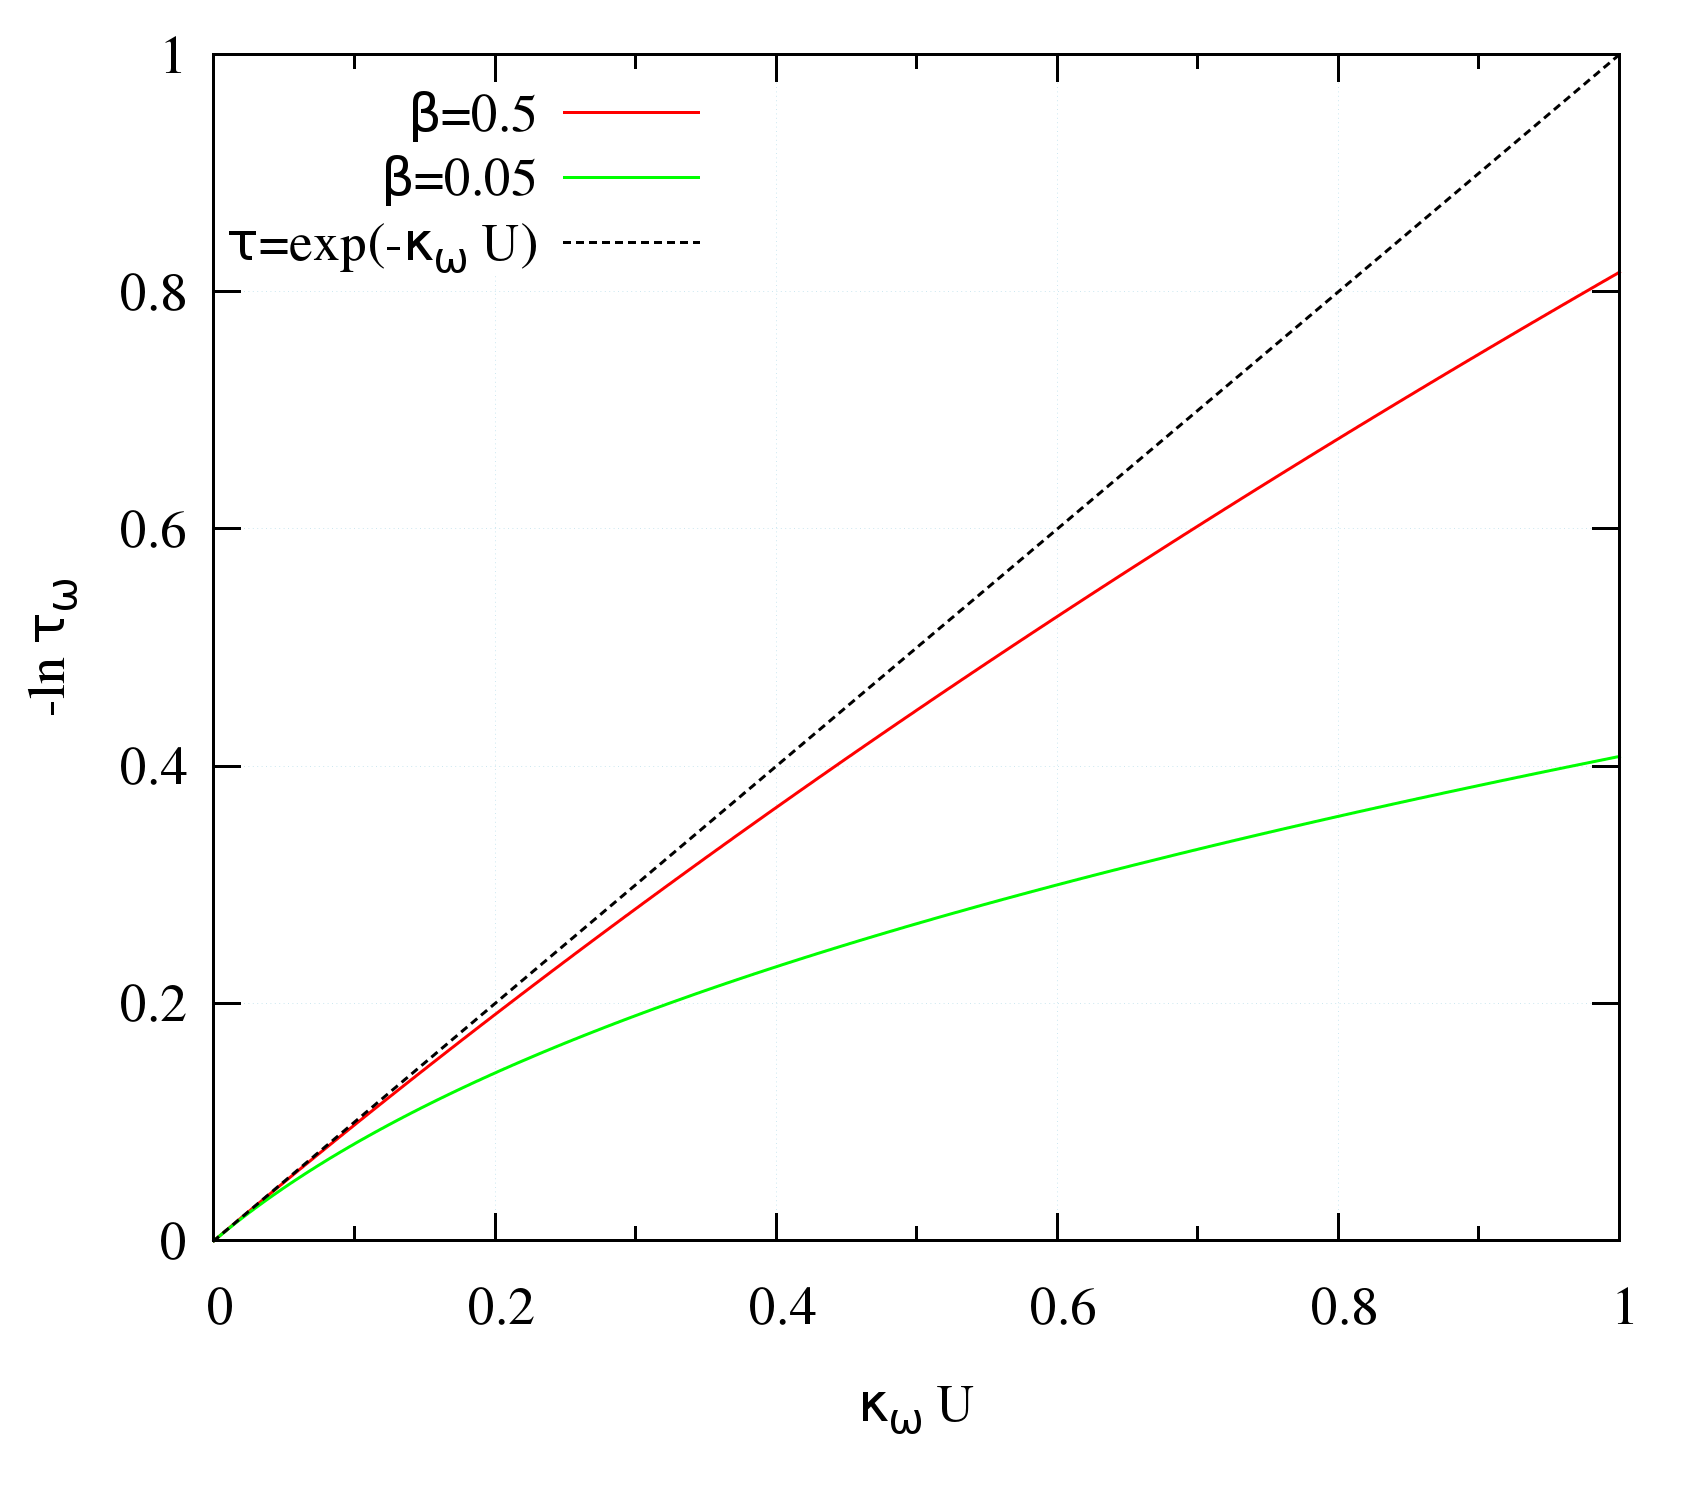
\includegraphics[width=4.0in]{Figures/Goody_curve_of_growth.png}
\end{center}
 \caption{Goody model curve of growth ($\ln \bar{\tau}$) as a function of the product $\bar{\kappa}_{\om}\;U$. Two different values of the overlap parameter are plotted: $\beta = 0.05$ (in green) and $\beta = 0.5$ (in red). The curve of growth for the ``weak line regime'' is also plotted (dashed curve).\label{fig::Goody_curve_growth}}
\end{figure}

\subsection{Malkmus model}\label{sec:malkmus_model}

Like the Goody model, the Malkmus model assumes the line strength of all the lines in a given narrow-band model follows a particular distribution. This model was developed because the exponential distribution assumed in the Goody model substantially underestimates the number of low-intensity lines. The Malkmus model is based on a more physical approach that assumes that the line strength distribution $P(S)$ varies proportionally to $S^{-1}$. This assumption is based on physical arguments and is empirically verified for some molecules, see Malkmus~\cite{Malkmus1967} for more details.

The problem of non-normalization of the $S^{-1}$ distribution is circumvented by cutting-off the $S^{-1}$ distribution below some very small and above some very large values of $S$. A continuous distribution can then be constructed based on some assumptions relating the energy of a transition with the line strength and assuming that the ratio between the maximum and the minimum line strengths considered is very large. The line strength probability distribution used in the Malkmus model is expressed by an exponential-tailed $S^{-1}$ distribution \cite{Malkmus1967,Young1977d}:
\begin{equation}
 P(S_E,S) = \dfrac{1}{S}\exp\left(-\dfrac{4}{\pi}\dfrac{S}{S_E} \right),
\end{equation}
where the effective line strength $S_E$ relates to the average line strength $\bar{S}$ through Eq.~\ref{eq::S_E_barS}. Solving Eq.~\ref{eq:SNB_tau_equiline}, and using the same definition for the effective average lines spacing $d_E$ as given in the above section, it comes:
\begin{align}\label{eq::Malkmus}
    \bar{\tau}_{\om} = \exp\left( -2 \dfrac{\gamma_c}{d_E} {\displaystyle \sqrt{1+\frac{S_E U}{\gamma_c }} -1 }\right) \nonumber \\
    \bar{\tau}_{\om} =  \exp\left(-2  \beta \left[\sqrt{1+\dfrac{\bar{\kappa}_{\omega}U}{\beta} }- 1\right] \right)
\end{align}
where the band overlap parameter $\beta$ is here again defined as:
\be
\beta = \dfrac{\gamma}{d_E} = \dfrac{\pi}{4}\dfrac{\gamma}{d}.
\ee

The Malkmus band model is recognized as the most suitable statistical narrow-band model for polyatomic gases \cite{Modest2013}. In this new version of RadCal, this model has been introduced to model the newly implemented fuel species. Note that the Malkmus and Goody models do not differ when considering the extreme cases of optically thin and optically thick medium. In such cases, both models asymptote to:
\begin{align}
\lim_{U \to 0} \dfrac{\bar{W}}{d}/U &= \bar{\kappa} \\
\lim_{U \to +\infty} \dfrac{\bar{W}}{d}/\sqrt{U} &= 2\displaystyle\sqrt{\bar{\kappa}\beta}
\end{align}

Figure~\ref{fig::Malkmus_curve_growth} plots the curve of growth, $-\ln(\bar{\tau}_{\om})$, versus the product $\bar{\kappa}_{\om} U$ for two different values of the overlap parameter: $\beta = 0.05$ (in green) and $\beta = 0.5$ (in red) using the Malkmus model. The back dashed curve corresponds to the ``linear'' behavior, \textit{i.e.} $\bar{\tau}_{\om} = \exp\left(-\bar{\kappa} U\right)$.

Again, it can be seen from Eq.~\ref{eq::Malkmus} that $\bar{\tau}_{\om}$ is fully characterized once the narrow-band parameters $\bar{\kappa}_{\om}$ and $\beta$ are known. These two narrow-band spectral quantities can be obtained either from line-by-line calculations, by fitting experimental data, or by physical considerations.

\begin{figure}
\begin{center}
 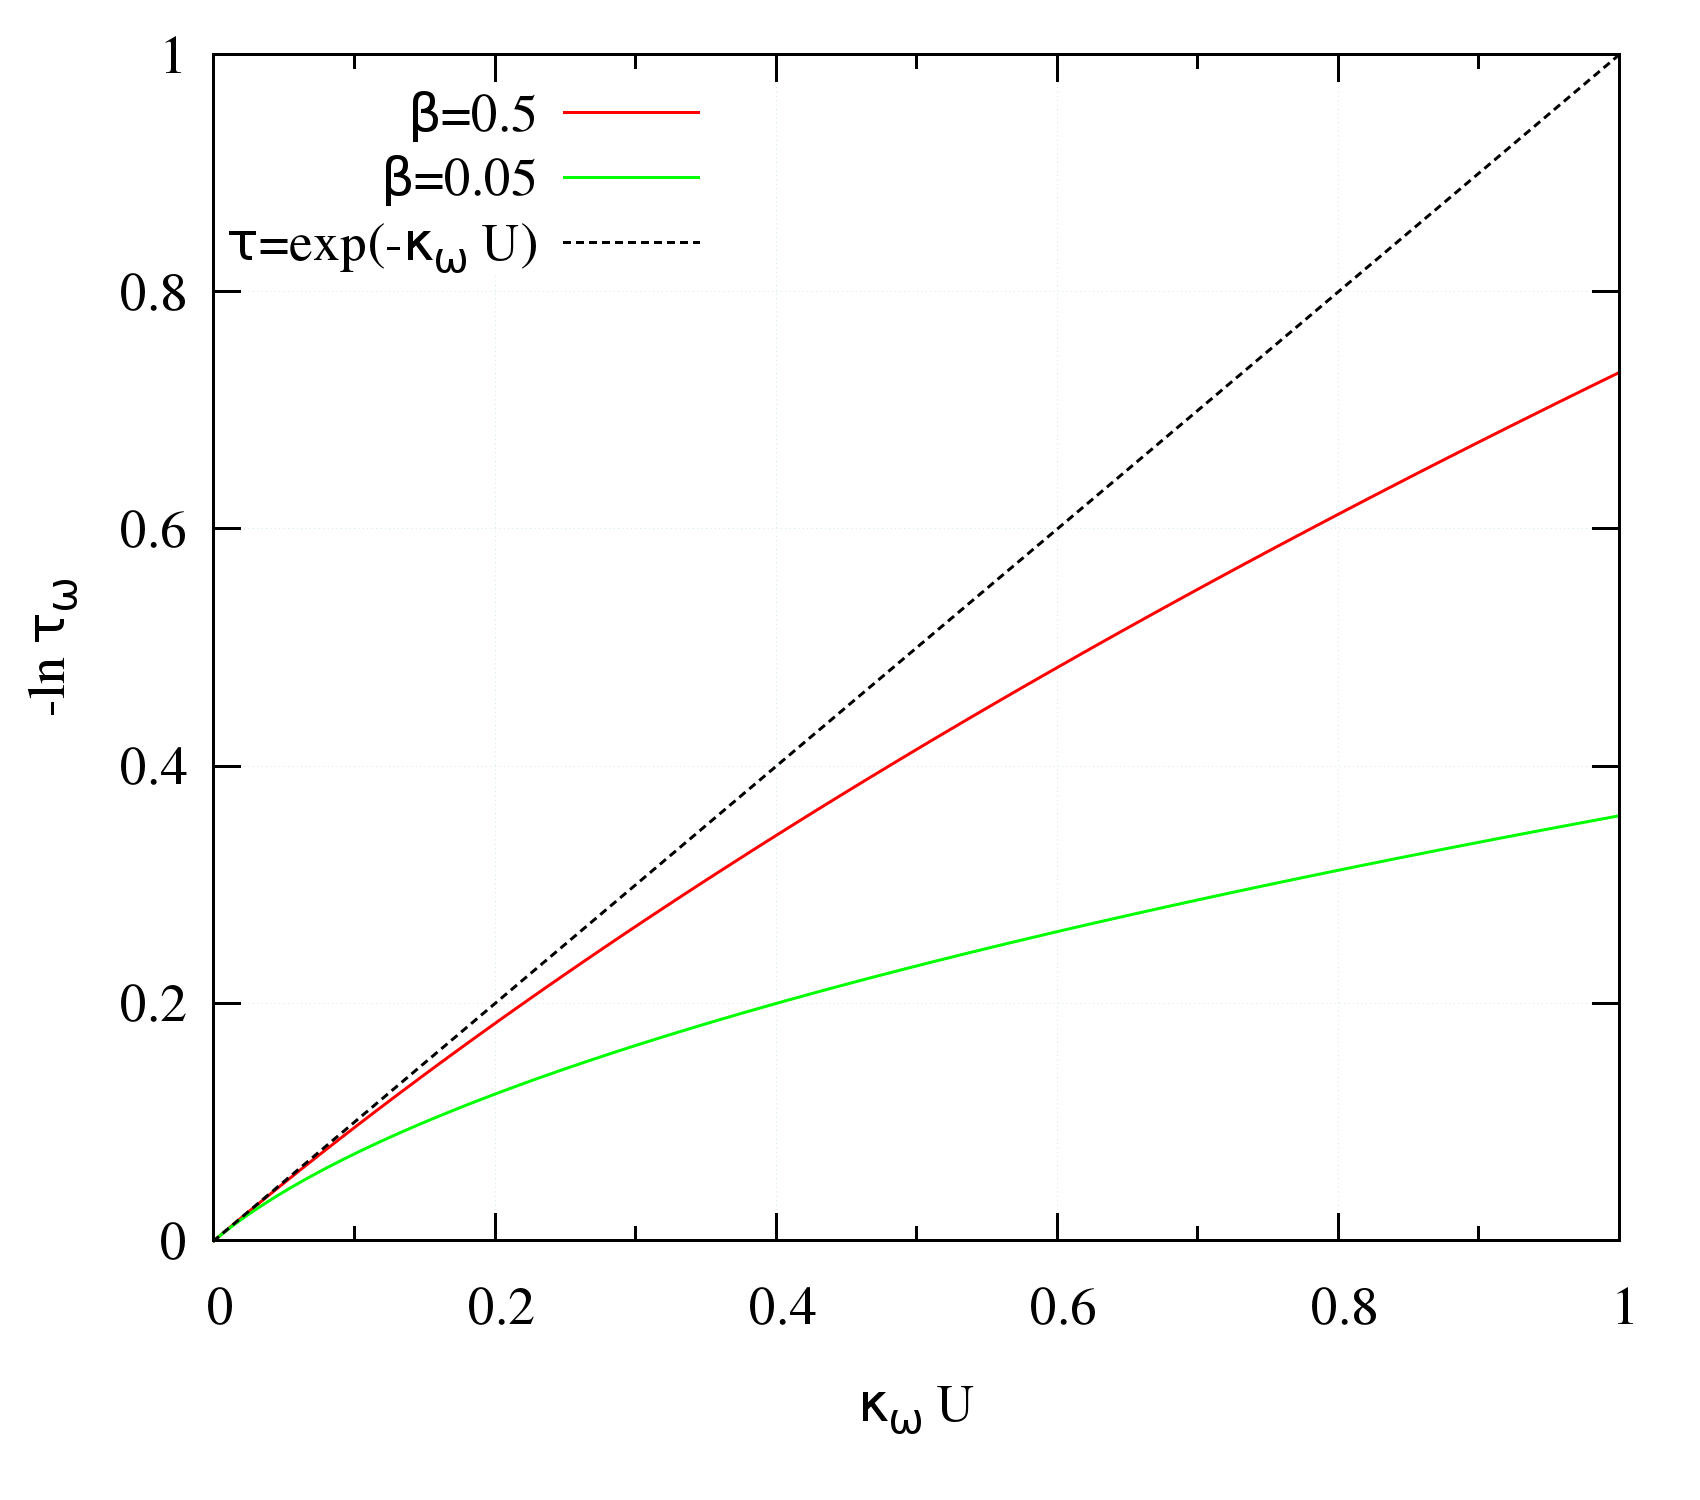
\includegraphics[width=4.0in]{Figures/Malkmus_curve_of_growth.png}
\end{center}
 \caption{Malkmus model curve of growth ($-\ln \bar{\tau}$) as a function of the product $\bar{\kappa}_{\om} U$. Two different values of the overlap parameter are plotted: $\beta = 0.05$ (in green) and $\beta = 0.5$ (in red). The curve of growth for the ``weak line regime'' is also plotted (dashed curve).\label{fig::Malkmus_curve_growth}}
\end{figure}

\textbf{Note}: For all the tabulated data, a linear interpolation of $\bar{\kappa}_{\om}$ and $\beta_{\om}$ in temperature and/or in wavenumber is performed by RadCal when necessary. If the temperature sought is out of the tabulated data range, then the data at the nearest temperature are used.

\section{Treatment of the RTE in the scope of narrow-band model}\label{sec:RTE_NB}
This section presents the expression of the different calculations performed by RadCal to numerically solve the Radiative Transfer Equation for a narrow-band. The Radiative Transfer Equation for a narrow-band is recalled below using wavenumbers:
\be\label{eq::RTE_Wavenumber}
\underbrace{I_{\om_0}(s)}_{\rm Received\:intensity\:in\:s}  = \underbrace{{I_{\rm b,\om_o}(T_w) \bar{\tau}(\om_0; 0 \rightarrow s)}}_{\rm transmitted\:incident\:intensity} + \underbrace{{\displaystyle\int_0^{s}{I_{\rm b,\om_0}\left(T(s')\right)\dfrac{\partial \bar{\tau}  }{\partial s'}(\om_0; s' \rightarrow s) \d s'}}}_{\rm intensity\:emitted\:by\:the\:medium\:between\:0\:and\:s}.
\ee
where $\Delta \om$ is the narrow-band centered in $\om_0$, $I_{\om_0}(s)$ is the received flux at the location $s$, $I_{b,\om_o}(T_w)$ is the incident flux penetrating the participating medium and which is modeled in RadCal as a flux from a blackbody of temperature $T_w$ ($T_w$ is an user input). The second term of the equation right-hand side accounts for the medium radiative emission and self-absorption.

\subsection{Treatment of Homogeneous pressure-path}
\label{sec::homogeneous_path}
If the participating medium is homogeneous -- \textit{i.e.} of constant composition, temperature $T$, and total pressure $P_T$ -- Eq.~\ref{eq::RTE_Wavenumber} can be simplified as:
\be\label{eq::RTE_wavenumber_H}
I_{\om_0}(s) = I_{\rm b,\om_o}(T_w) \bar{\tau}(\om_0; 0 \rightarrow s) + I_{\rm b,\om_o}(T)(1-\bar{\tau}(\om_0; 0 \rightarrow s)).
\ee
RadCal computes the value of $\bar{\tau}(\om_0; 0 \rightarrow s)$ combining Lorentz and Doppler lines. While usually for cases at atmospheric pressure and at moderate temperature the Doppler lines are not important, they are however included for the sake of completeness. The different steps of the calculation of $\bar{\tau}(\om_0; 0 \rightarrow s)$ are presented below.

For each participating species present in the medium, RadCal first retrieve the band mean absorption coefficient $\bar{\kappa}_{\om}$, the band overlap parameter $\beta$ (for Lorentz lines), and the Doppler fine structure parameter, denoted $a_D$, which is defined as the ratio of the Doppler HWHM $\gamma_D$, given by Eq.~\ref{eq::DopplerHWHM}, over the mean line spacing $d$.

Then RadCal computes the optical depth from Lorentz lines, denoted $X_C$, using Eqs.~\ref{eq::Elsasser}, \ref{eq::Goody}, and \ref{eq::Malkmus}, depending on the species appropriate model, using  $\bar{\kappa}_{\om}$ and $\beta$. Note that:
\be\label{eq::Collision_optical_depth}
X_C = \dfrac{\bar{W}}{d}
\ee

RadCal computes the optical depth from Doppler lines, denoted $X_D$. The expression of $X_D$ depends of the model chosen to compute $X_C$. If the Elsasser or Goody model is used to compute $X_C$, then the optical depth from Doppler lines is calculated by \cite{Ludwig1973}:
\be\label{eq::Doppler_optical_path_Goody}
X_D = \sqrt{\dfrac{2}{\ln 2}} a_D \sqrt{\ln \left(1+\dfrac{\ln 2}{2} \left(\dfrac{\bar{\kappa}_{\om_0}U}{a_D}\right)^2\right)},
\ee
where $U$ is the optical thickness defined by $U = P_i\,s$, with $P_i$ the partial pressure (in atm) of the participating species considered and $s$ is the distance given in cm.
If the Malkmus model is used to compute $X_C$, then the optical depth from Doppler lines is calculated by \cite{Ludwig1973}:
\be\label{eq::Doppler_optical_path_Malkmus}
X_D = \sqrt{\dfrac{3}{2 \ln 2}} a_D \left[ \ln\left(1 + \left(\sqrt{\dfrac{2 \ln 2}{3}} \dfrac{\bar{\kappa}_{\om_0}U}{a_D} \right)^{2/3} \right)\right]^{3/2}.
\ee
The combined optical depth, $Y$, is then calculated:
\be\label{eq::combined_optical_path}
Y  = \left(1 - \left(\dfrac{X_C}{\bar{\kappa}_{\om_0}U}\right)^2 \right)^{-2} + \left(1 - \left(\dfrac{X_D}{\bar{\kappa}_{\om_0}U}\right)^2 \right)^{-2} - 1.
\ee
Finally, the narrow-band transmissivity, $\bar{\tau}(\om_0; 0 \rightarrow s)$, is obtained by:
\be\label{eq::trans_HPP_final}
\bar{\tau}(\om_0; 0 \rightarrow s) = \exp\left(-\bar{\kappa}_{\om_0}U \sqrt{1 - \dfrac{1}{\sqrt{Y}}}\right).
\ee
If there are more than one participating species, then $\bar{\tau}(\om_0; 0 \rightarrow s)$ is calculated from:
\be\label{eq::trans_HPP_final_multispecies}
\bar{\tau}(\om_0; 0 \rightarrow s) = \exp\left(-\displaystyle\sum_i{\bar{\kappa}_{i,\om_0}U \sqrt{1 - \dfrac{1}{\sqrt{Y_{i}}}}}\right),
\ee
the optical depth for each species $i$ is first calculated separately, and then summed altogether.

\subsection{Treatment of non-Homogeneous pressure-path - Curtis-Godson approximation}
\label{sec::Curtis_Godson}
The treatment of the RTE in the case of non-homogeneous medium (where gradients of species, temperature, or pressure are present) is explicitly detailed below. The non-homogeneous case is first treated by discretizing the depth of penetration of the incident beam of direction $\hat{\textbf{s}}$ into a set of $n$ smaller segments $\{[s_{i-1};s_i]\}_n$ over which the local composition, temperature, and pressure can reasonably be assumed constant. Hence, the expression of the RTE over a narrow-band $\Delta \om$, centered in $\om_0$ and given by Eq.~\ref{eq::RTE_Wavenumber} can be simplified as:
\begin{equation}\label{eq::RTE_wavenumber_NH}
I_{\om_0}(s) = I_{\rm b,\om_o}(T_w) \bar{\tau}(\om_0; 0 \rightarrow s) + \displaystyle\sum_{i=1}^n{I_{\rm b,\om_o}(T_i)\left(\bar{\tau}(\om_0; s_i \rightarrow s)-\bar{\tau}(\om_0; s_{i-1} \rightarrow s)\right)}.
\end{equation}
In the expression, it assumed that $s_0 = 0$, which is coincided with the location of the blackbody wall of temperature $T_w$, and $s_n = s$. The temperature $T_i$ is the temperature of the small segment $\{[s_{i-1};s_i]\}_n$. The difficulty in solving Eq.~\ref{eq::RTE_Wavenumber} lies in evaluating  $\bar{\tau}(\om_0; s_i \rightarrow s)$ as it is correlated with the cells crossed by the beam $\widehat{\textbf{sis}}$.

To circumvent this difficulty, the Curtis-Godson approach is used. In this approach, it is assumed that
each $\bar{\tau}(\om_0; s_i \rightarrow s)$ for a given species can still be calculated using Eqs.~\ref{eq::Doppler_optical_path_Goody}, \ref{eq::Doppler_optical_path_Malkmus}, \ref{eq::combined_optical_path}, \ref{eq::trans_HPP_final}, and the models presented in Section~\ref{Sec::SNBM} but their parameters $\bar{\kappa}$, $\beta$, and $a_D$ are replaced by some effective parameters, $\bar{\kappa}^*$, $\beta^*$, $a_{D}^*$, respectively. See Young \cite{Young1977d} and Ludwig \textit{et al.} \cite{Ludwig1973} for additional details on the Curtis-Godson approach. It was found that using path-averaged parameters as effective parameters work best \cite{Young1977d} to calculate the transmissivity of non-homogeneous medium. These parameters are defined as:
\begin{align}
\bar{\kappa}^* &= \dfrac{\displaystyle\int_{s_i}^{s} \bar{\kappa}(s')P_i(s')\d s'}{\displaystyle\int_{s_i}^{s} P_i(s')\d s'}, \label{eq::effective_kappa} \\
\beta^* &= \dfrac{\displaystyle\int_{s_i}^{s} \beta(s')\bar{\kappa}(s')P_i(s')\d s'}{\displaystyle\int_{s_i}^{s} \bar{\kappa}(s')P_i(s')\d s'}, \label{eq::effective_beta}\\
a_D^* &= \dfrac{\displaystyle\int_{s_i}^{s} a_D(s')\bar{\kappa}(s')P_i(s')\d s'}{\displaystyle\int_{s_i}^{s}, \bar{\kappa}(s')P_i(s')\d s'},\label{eq::effective_ad}
\end{align}
with $P_i$ is the partial pressure of the participating gas considered. The quantity:
\be
U = \displaystyle\int_{s_i}^{s}{P_i(s')\d s'},
\ee
is the optical thickness, in {\rm atm.cm}, between the points $s_i$ and $s$.

\section{Output quantities: effective coefficients and integrated quantities}\label{sec::Output}
RadCal solves the RTE based on the input parameters found in the input file \verb=RADCAL.in= and returns in a Tecplot file (\verb=<CASE ID>.tec=, where \verb=<CASE ID>= is an user input defined in the input file) the spectral profile of the spectral transmissivity of the medium $\bar{\tau}(\om_0; 0 \rightarrow s)$ and the incident spectral intensity $I_{\om_0}(s)$ calculated using either Eq.~\ref{eq::RTE_wavenumber_H} or \ref{eq::RTE_wavenumber_NH}.

In addition to the Tecplot file, RadCal also generates an output file \verb=RADCAL.out=, that contains several effective coefficients and integrated quantities. Some of these integrated quantities were already included in the previous version of RadCal. This is the case of the effective absorption coefficient, the Planck mean absorption coefficient, and the received total directional radiative energy flux (or received total intensity). Two new integrated quantities have been added: the total emissivity, and the total transmissivity. These effective coefficients and integrated quantities are described formally in this section. Note that the integration is performed using a Simpson rule over non regular abscissa using a 3-point Lagrangian interpolation (quadratic interpolation).

\subsection{Effective absorption coefficient}
The path-averaged or effective absorption coefficient, denoted here $\kappa_{\rm e}$ and denoted \verb=Amean= in the output file, is defined such that the received total intensity in $s = L$ can be expressed as a sum of a transmitted total intensity coming from the blackbody wall, set at temperature $T_w$, and a total intensity emitted by the gas at the local temperature $T_g$:
\be\label{eq:effective_epsilon1}
   \int_{\om_{\rm min}}^{\om_{\rm max}}{I_{\om}(L) \; \d \om} = \exp\left(-\kappa_{\rm e}\, L\right) \int_{\om_{\rm min}}^{\om_{\rm max}}{ I_{\rm b,\om}(T_w) \; \d \om} + \left(1-\exp\left(-\kappa_{\rm e} \, L\right)\right) \int_{\om_{\rm min}}^{\om_{\rm max}}{I_{\rm b,\om}(T_g) \; \d \om}
\ee
where $L$ is the total path length given in cm. The bounds of integration in Eq.~\ref{eq:effective_epsilon1} are fixed, with $\om_{min} = 5$ cm$^{\rm -1}$, and $\om_{max} = 25000$ cm$^{\rm -1}$. However, the bounds of the integration for the gas-phase species are specified by the user. The remain outside spectral domain is integrated then considering only the contribution of soot (if present). See Eq.~\ref{eq::received_flux}. The large bounds of integration (5 -- 25000 cm$^{\rm -1}$) is large enought such that:
\be
\int_{\om_{\rm min}}^{\om_{\rm max}}{I_{b,\om}(T) \; \d \om} \approx \dfrac{\sigma}{\pi}T^4.
\ee

Formally, $\kappa_{\rm e}$ is calculated from:
\be\label{eq:effective_epsilon}
   \kappa_{\rm e} = -\dfrac{1}{L} \ln\left(\dfrac{\displaystyle\int_{\om_{\rm min}}^{\om_{\rm max}}{I_{\om}(L)  - I_{\rm b,\om}(T_g)\; \d \om}   }{\displaystyle\int_{\om_{\rm min}}^{\om_{\rm max}}{ I_{\rm b,\om}(T_w)-I_{\rm b,\om}(T_w) \; \d \om}  } \right).
\ee
Note that $\kappa_{\rm e}$ has the units of cm$^{-1}$. The effective absorption coefficient is calculated for homogeneous and non-homogeneous cases. For the latter, the gas temperature $T_g$ used in Eq.~\ref{eq:effective_epsilon} is the path-average temperature:
\be\label{eq::Path_avg_temp}
T_g = \dfrac{\displaystyle\int_{0}^{L}{T(s) \d s }}{L}.
\ee
While the effective absorption coefficient works well for a given length $L$, one has to be careful when using it to estimate the received total intensity from a similar homogeneous isothermal medium but with a different thickness as the calculated results using Eq.~\ref{eq:effective_epsilon} might deviate significantly from the actual results unless the medium considered is gray (no spectral variation of the absorption coefficient).

\subsection{Planck mean absorption coefficient}
The Planck mean coefficient, denoted here $\kappa_{\rm Planck}$, is calculated by:
\begin{equation}\label{eq::planck_mean}
\kappa_{\rm Planck} = \dfrac{\pi}{\sigma {T_g}^4}
\displaystyle\int_{\om_{\min}}^{\om_{\max}}{I_{\rm b,\om}(T_g)
\displaystyle\sum_i \bar{\kappa}_{i,\om} \, P_i \; \d \om}
\end{equation}
where $P_i$ is the partial pressure of participating species $i$, in units of ${\rm atm}$; and $\bar{\kappa}_{\om}$ is the narrow-band mean absorption coefficient of participating species $i$, in units of ${\rm atm^{-1}.cm^{-1}}$. Note that the temperature used in this expression is the local gas temperature; thus, $\kappa_{\rm Planck}$ is a function of the gas phase temperature and of the species partial pressure. It is independent of the path physical length. Its units are in ${\rm cm^{-1}}$. The integration bounds, $\om_{min}$, and $\om_{max}$ are defined by the user in the input file.

The Planck mean absorption coefficient is calculated for homogeneous and non-homogeneous cases. For the latter, the gas temperature used to calculate $I_{\rm b,\om}(T_g)$ is the path-average temperature as defined by Eq.~\ref{eq::Path_avg_temp}. The term $T_g^4$ is also calculated using a path-average value:
\be
T_g^4 = \dfrac{\displaystyle\int_{0}^L{ T(s)^4 \d s}}{L},
\ee
where $L$ is the total path length given in cm.

For non-homogeneous cases, the mean absorption coefficient used in Eq.~\ref{eq::planck_mean}, $\bar{\kappa}_{i,\om}$, corresponds to the effective mean absorption coefficient $\bar{\kappa}^*$ defined by Eq.~\ref{eq::effective_kappa}. The partial pressure used is a path-average partial pressure:
\be
P_i = \dfrac{\displaystyle\int_{0}^L{P_i(s)\d s}}{L}.
\ee

\subsection{Total transmissivity}

Radcal returns the total transmissivity, denoted $\tau_{T}$, of the spectral range bounded between the user defined $\omega_{min}$ and $\omega_{max}$. The total transmissivity is calculated as:
\begin{equation}\label{eq::total_transmissivity}
 \tau_{T} = \dfrac{\displaystyle\int_{\omega_{min}}^{\omega_{max}}\tau(0 \rightarrow s;\omega)I_{\rm b,\om}(T_w) \d \omega }{\displaystyle\int_{\omega_{min}}^{\omega_{max}}I_{\rm b,\om}(T_w)\d \omega }.
\end{equation}
This quantity is dimensionless. It represents the fraction of transmitted incident intensity from the blackbody wall set at temperature $T_w$. It is worth noting that since it depends on $T_w$, changing $T_w$ while keeping constant all the other simulation parameters will yield different values of $\tau_{T}$.

\subsection{Total emissivity}

Radcal returns the total emissivity, denoted $\varepsilon_{T}$, for the spectral range bounded by the user defined $\omega_{min}$ and $\omega_{max}$. It is derived from the effective absorption coefficient $\kappa_{\rm e}$ through:
\begin{equation}\label{eq:total_emissivity}
\varepsilon_{T} = 1 - \exp\left(- \kappa_{\rm e} L \right),
\end{equation}
where $L$ is the total physical length of the participating layer, given in $\rm cm$. The total emissivity is dimensionless.

\subsection{Received flux}
RadCal returns the integrated value of the received total directional radiative energy flux (or received total intensity), denoted \verb=Received Flux= in \verb=RADCAL.out= file. The integration is performed between the user defined bounds $\omega_{min}$ and $\omega_{max}$. Note that contribution of soot (if present) is added in the ranges 5~$\rm cm^{-1}$ to $\om_{min}$ and $\om_{\max}$ to 25,000~$\rm cm^{-1}$. Its units are in $\rm W.m^{-2}.str^{-1}$. The received total intensity, denoted $I(L)$, is calculated by:
\be\label{eq::received_flux}
I(L) = \underbrace{\displaystyle\int_{\om_{min}}^{\om_{max}}{I_{\om}(L)\d \om}}_{\rm All\:species} + \underbrace{\displaystyle\int_{5}^{\om_{min}}{I_{\om}(L)\d \om}}_{\rm Soot\:only} +  \underbrace{\displaystyle\int_{\om_{max}}^{25,000}{I_{\om}(L)\d \om}}_{\rm Soot\:only},
\ee
where $I_{\om}(L)$ is obtained from Eq.~\ref{eq::RTE_wavenumber_H} for homogeneous cases, and Eq.~\ref{eq::RTE_wavenumber_NH} for non-homogeneous cases.
